\chapter{Probing for phonological representations in phoneme LMs}\label{chapter:phonology}

Language models provide a key framework for studying linguistic theories based on prediction, but phonological analysis using LMs is difficult. Standard benchmarks are generally based on higher-order structures: syntax and semantics, rather than morphology and phonology. Small models trained on developmentally plausible data are useful tools for linguistic analysis, as introduced in \cref{sec:12-plausiblepretraining}, but most of this work involves training on orthographic text with a subword-based input representation, restricting the ability to study phonological representations and word learning. \Cref{chapter:modelling} established the feasibility of training BabyLMs with a phoneme-based input representation, evaluated using the BabySLM benchmark, but as with many other evaluation benchmarks, BabySLM only supports English evaluation.

This chapter introduces language-independent methods for phonological probing. These methods are applied to phoneme LMs trained on the 31 languages in \ipachildes, described in \cref{sec:15-suite}. First, in \cref{sec:15-wordseg}, the word segmentation task is used to explore whether phoneme LMs implicitly track word boundaries to aid in prediction. Following past models of word segmentation, a set of unsupervised methods for the word boundary task are introduced, as well as linear probes to investigate whether word boundaries are encoded by these models. Following these, \cref{sec:15-featureprobing} leverages linear probes to investigate whether distinctive phonological features are encoded, despite the model only having distributional cues to learn from. The results of these methods provide new insights for distributional phonology and language model interpretability,as discussed in \cref{sec:15-discussion}.

% This chapter demonstrates how probing the phonological representations in phoneme LMs trained on developmentally plausible phonemic transcripts can lead to new insights across distributional phonology and language model interpretability. A suite of phoneme LMs are trained on the 31 languages in \ipachildes and the representations are probed using two tasks. First, using the corresponding entries in \phoible, the models are probed for phonological features. 

% First, phoneme LMs trained on 11 languages in \ipachildes are probed for phonological features (which can be easily accessed in the \phoible database due to the folding maps used by \gpp). Secondly, the word segmentation task is used to investigate whether phoneme LMs trained without word boundaries implicitly track them to aid in prediction. For this task, linear probes are used, but also unsupervised methods --- the success of the later corroborating statistical learning theories of acquisition and empirically motivates new methods for training subword tokenisers.

% \section{Representations of word boundaries in LMs}\label{sec:15-background}

% In this study, we combine ideas from past computational models for word segmentation. Rather than explicitly calculate n-gram statistics, our cues are based on prediction-error and utterance boundary probability extracted from LLMs trained on the next-phoneme prediction task. As these cues are based on the language model's prediction of phonemes, successful segmentation indicates that implicit phonological knowledge of word-like units in these models. 

% In this work, we explore the phonological capabilities of phoneme-based BabyLMs across 31 languages using the \textbf{word segmentation task}. Following the computational models of word segmentation introduced in \cref{sec:12-wordseg}, models are assessed by their ability to correctly place word boundaries in a sequence of phonemes when word boundaries are not provided during training. Successful segmentation indicates implicit phonological knowledge and when performed zero-shot on developmentally plausible data, contributes to statistical learning theories of language acquisition. 

% In some of the earliest sequential models, it was noted that \emph{prediction-error} (the degree to which the model struggles to predict the next token) often corresponded with word boundaries \citep{elman-1990-finding}. Using this observation,
% %Noting that prediction-error in sequential models indicates word boundaries \citep{elman-1990-finding}, 
% we identify four word boundary cues that can be extracted from trained models and three unsupervised strategies for placing boundaries using these cues, as illustrated in \cref{fig:15-example}. We additionally follow the supervised approach of \citet{hahn-baroni-2019-tabula}, training linear probes on final layer embeddings to determine if word boundaries are implicitly tracked in order to improve phoneme prediction.

% We train phoneme-based BabyLMs on the phonemic transcriptions of child-centred speech comprising the \ipachildes dataset \citep{goriely2025}. We find that these models implicitly encode word boundaries across all 31 languages and identify two factors that may provide useful priors depending on the language: the length of words and the distribution of phonemes at the end of words. 

% %but that word-final phoneme distributions and word lengths vary between languages and act as confounding factors, making it difficult to compare results across languages. 

% We discuss the validity of orthographic word boundaries as gold labels and note the similarities between our results and recent work that uses byte-level prediction entropy to improve the tokenization step in large language model (LLM) pre-training \citep{pagnoni2024byte}. We conclude that this framework not only supports the study of distributional phonology and acquisition, but could also have implications for improving the efficiency and robustness of LLMs.

\section{A suite of cross-lingual phoneme LMs}\label{sec:15-suite}

In order to study the phonological representations of phoneme LMs cross-lingually, \gpt models are trained on each of the 31 languages in \ipachildes. Since the smallest section (Farsi) only contains \q{40}{\thousand} words of child-directed speech, for a fair comparison, every other section must be subsampled, and a small model must be used to prevent over-fitting. In order to explore the phonological representations learned by larger models trained with more data, four suites of models are trained, each using a different sample size and model size. The model parameters for subsample size are chosen according to the scaling experiment results in \cref{chapter:modelling} --- using the parameters that led to the highest BabySLM lexical score.

These parameters are summarised in \cref{tab:15-suites}. The Tiny suite contains models trained on just \q{20}{\thousand} tokens from each of the 31 languages in \ipachildes, whereas the Large suite consists of just one model trained on \q{18}{\million} tokens of the EnglishNA section. These suites are referred to as ``cross-lingual'' since each individual model is monolingual, only trained on data from a single language. This is in contrast to ``multilingual'' models that are trained on multiple languages at once.

%During training, we reserve 5000 tokens from each language to use for evaluation, kept consistent across suite sizes.
\setlength{\tabcolsep}{2pt}
\begin{table}[t]
    \centering
    \small
    \begin{tabular}{rccc}
    \toprule
        Suite Size & Model Parameters & Tokens (words) & Languages \\
       \midrule
       Tiny & 400k & 100k (20k) & 31 \\
       Small & 600k & 700k (180k) & 17 \\
       Medium & 5M & 1.8M (500k) & 11 \\
       Large & 19M & 18M (5M) & 1 \\
       \bottomrule
    \end{tabular}
    \caption{The model size in number of (non-embedding) parameters and data size used for each suite of models. Languages are subsampled according to the token count for consistency, as word length varies across languages. Word counts provided are estimates. The model sizes were chosen according to the results in \cref{tab:14-bestsizes} and full parameters are detailed in \cref{tab:14-model_sizes}.}
    \label{tab:15-suites}
\end{table}

\section{Experiment: Probing for word boundaries}\label{sec:15-wordseg}

Previous work has explored the representations of word boundaries in LMs. \citet{sanabria2021difficulty} explored methods for extracting word boundaries from attention weights in an LSTM, finding that attention had limited value for segmentation. \citet{hahn-baroni-2019-tabula} trained character-level RNNs and LSTMs without word boundaries, finding that individual activations correlated with word boundaries and that a linear probe trained on all activations also identified boundaries. They claim that removing word boundaries results in a `near tabula rasa' training paradigm, but train their models on billions of orthographic words from Wikipedia, which is not developmentally plausible.  %Here, we use this probe on the final layer of phoneme LMs trained on developmentally plausible data, a more `tabula rasa' paradigm. 

\begin{figure}[t]
    \centering
    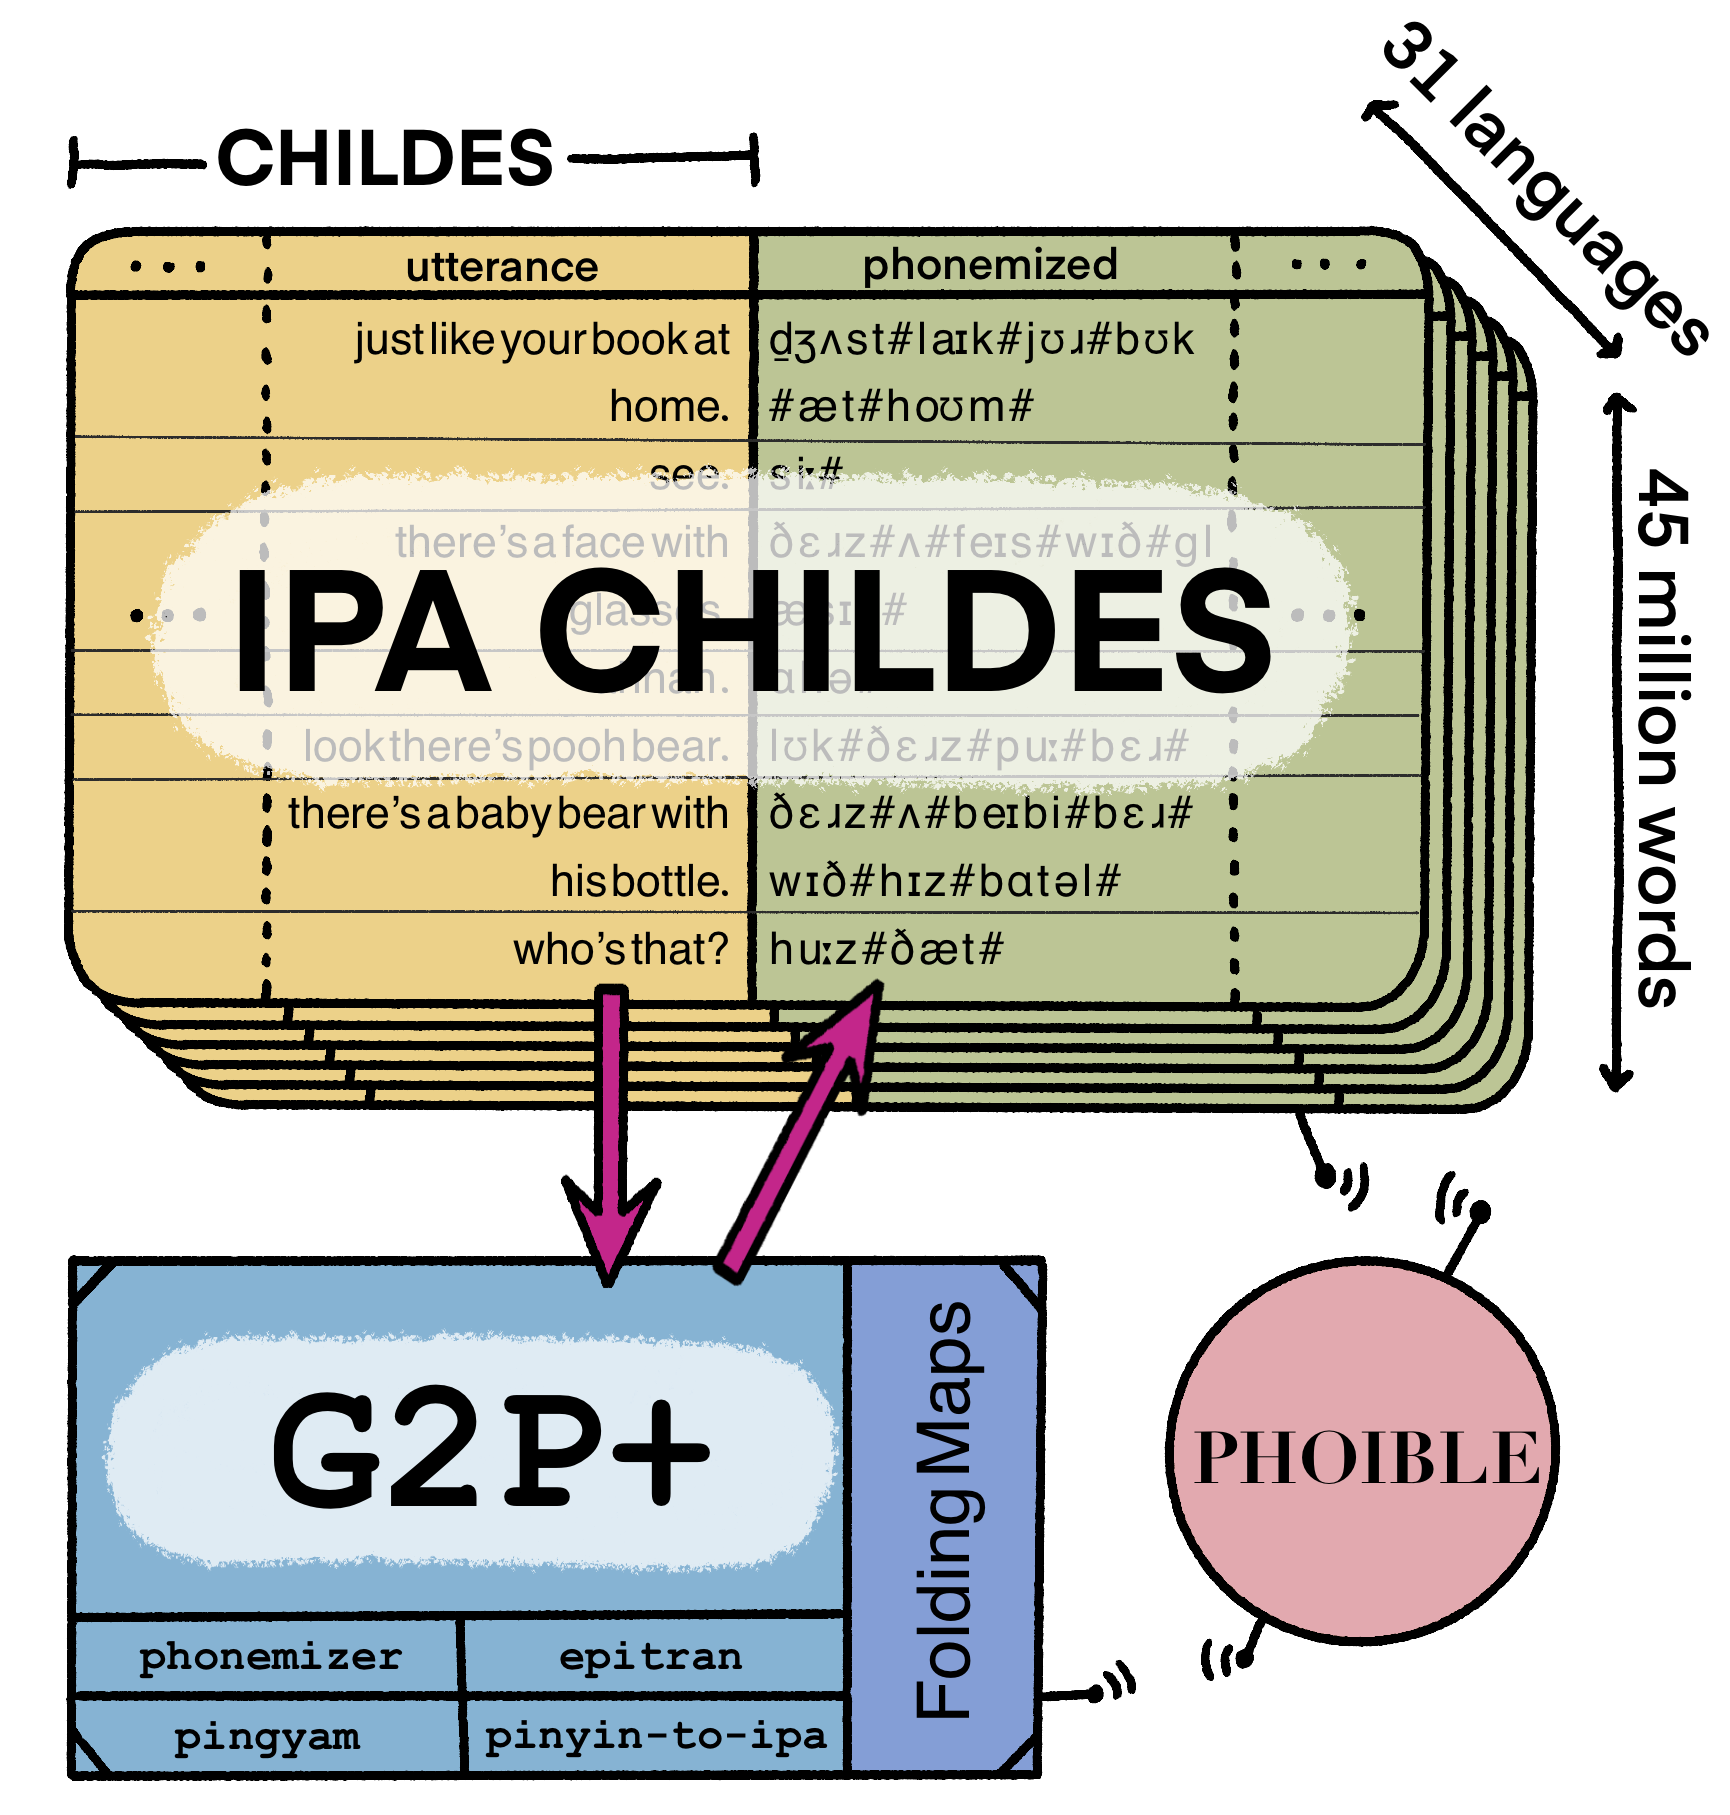
\includegraphics[width=0.7\linewidth]{15Phonology/overview.png}
    \caption{Three strategies for unsupervised word segmentation using cues extracted from an autoregressive language model trained to predict phonemes.}
    \label{fig:15-example}
\end{figure}

Here, word boundaries are extracted from phoneme LMs trained on child-directed speech transcripts, a more `tabula rasa' paradigm. Two methods for extracting word boundaries are explored; an unsupervised method that follows past computational models of word segmentation (as introduced in \cref{sec:12-wordseg}) and a linear probe, following \citet{hahn-baroni-2019-tabula}.

\subsection{Unsupervised word segmentation}\label{sec:15-wordsegunsupervised}

Given a list of utterances, each of which consists of a non-delimited phoneme sequence, the task of an unsupervised word segmentation method is to produce a \emph{segmentation} of each utterance by using an unsupervised method for placing word boundaries. For instance, given the utterance ``what do you see'', represented phonemically as \ttipa{w2tdu:yu:si:}, successful segmentation would return \ttipa{w2t du: yu: si:}, as demonstrated in \cref{fig:15-example}.

The unsupervised word segmentation method is based on the observation made by \citet{elman-1990-finding}, that cues for word boundaries can be extracted from a sequence prediction model. Given a language model that at each position $i$ provides the probability of a phoneme $x$ given a context $x_1\ldots x_{i-1}$, the following four cues are extracted at each potential boundary position:

\begin{itemize}[leftmargin=*]
    \item \textbf{Entropy:} The entropy (in bits) across the probabilities for all items in the vocabulary.%\footnote{The vocabulary consists of all phonemes and a dedicated utterance boundary token.}
    \item \textbf{Surprisal:} The negative log probability of the subsequent phoneme $p_i$, measured in bits. %cross-entropy loss (bits) 
    \item \textbf{Rank:} The rank of $x_i$ in the list of possible tokens at position $i$ sorted by likelihood.
    \item \textbf{Utterance Boundary Probability (UBP):} The probability assigned to the utterance boundary token.
\end{itemize}

The first three cues are put forward by \citet{al-rfou_character-level_2019}, where they are used to qualitatively examine the error rate of their character-based language model. Note that in their study, the surprisal cue is called loss, but surprisal is equivalent to cross-entropy loss in auto-regressive language models. Here, these cues are used in a novel way to extract word boundaries. The fourth cue, UBP, relates to the model of \citet{christiansen1998learning}, who found that the prediction of the utterance boundary marker in a SRN increased at word boundaries. Similar cues have been utilised in the segmentation models of \citet{ccoltekin2014explicit} and my previous study \citep{goriely2023word} --- but in these, they were calculated using n-gram frequencies, whereas here, they are calculated using the probability distribution produced by a phoneme LM.

For each of these cues, three methods are introduced for placing word boundaries. The first is to identify peaks in each cue: placing word boundaries whenever the cue's value is higher at position $i$ than at position $i-1$ or $i+1$ in the sequence. The second is to learn a single threshold value, placing word boundaries when the cue exceeds it. The third combines both strategies, placing word boundaries when the relative increase of the cue's value from position $i-1$ to $i$ exceeds a learned threshold. These are called these the \textbf{peak}, \textbf{threshold} and \textbf{relative} strategies, respectively, as illustrated in \cref{fig:15-example}. Note that the threshold and relative strategies are not fully unsupervised, but only need to learn a single parameter. %While threshold segmentation is not technically unsupervised, it solves an issue with peak segmentation --- the failure to place two boundaries in sequence, despite some words consisting of a single phoneme.

For each model in each suite, each unsupervised strategy with each cue is used to segment a held-out set of utterances from \ipachildes corresponding to the language used to train that model. Following past work, word segmentation performance is reported using the \fscore of boundary placement, excluding boundaries placed at the start and end of utterances (as these are `free' from the utterance boundaries).

\subsection{Word boundary probe}

In addition to the unsupervised word segmentation methods, a linear probe is also used to extract word boundaries. Whereas the unsupervised method aligns with past segmentation models in demonstrating whether distributional information can be leveraged to group phonemes into words, linear probes can reveal whether a language model will implicitly track word boundary information in each phoneme representation in order to aid prediction. 

For each model in each suite, a linear probe is trained on embeddings taken from an equal number of word-final and word-internal positions, ensuring that no words in the training set are contained in the test set. This matches the `balanced' probe described by \citet{hahn-baroni-2019-tabula}. Each probe is trained on \q{1}{\thousand} contextual embeddings and tested on \q{10}{\thousand}. Given that the training data is balanced, accuracy is used to report the performance of these probes. \citet{hahn-baroni-2019-tabula} claim that chance performance is 50\% due to the balanced training data, but the results below suggest otherwise. All probes for a particular language are trained and tested on the same evaluation set. 

\subsection{Results}

\begin{figure}[t]
    \centering
    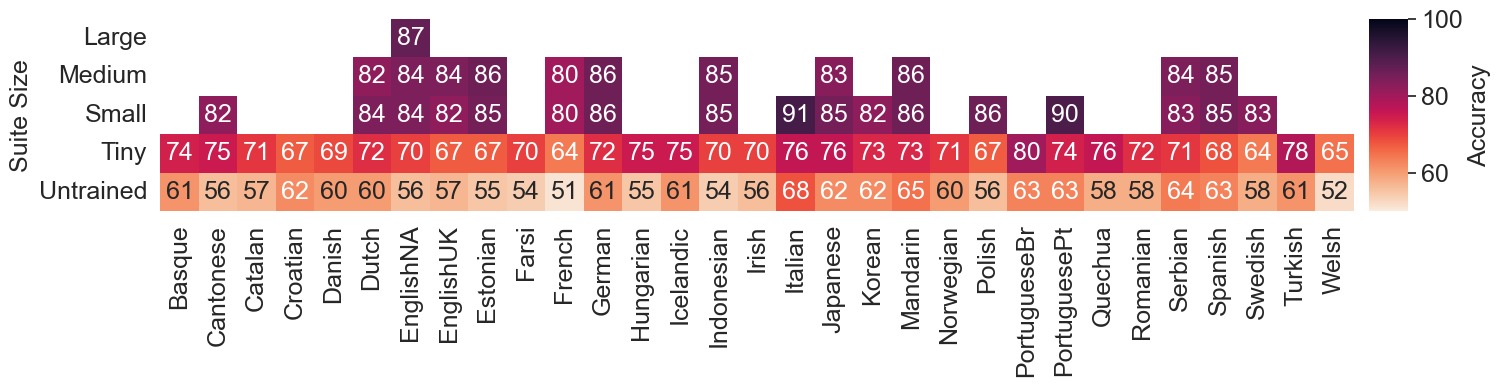
\includegraphics[width=\linewidth]{15Phonology/probe_results.png}
    \caption{Accuracy scores for the word boundary probe trained on the contextual embeddings of phonemes across models in each suite. Training and test instances are balanced and each word used for training embeddings is removed from the test set. Probe results for each untrained model in the Tiny suite are included as a baseline.}
    \label{fig:15-probes}
\end{figure}

\begin{figure}[t]
    \centering
    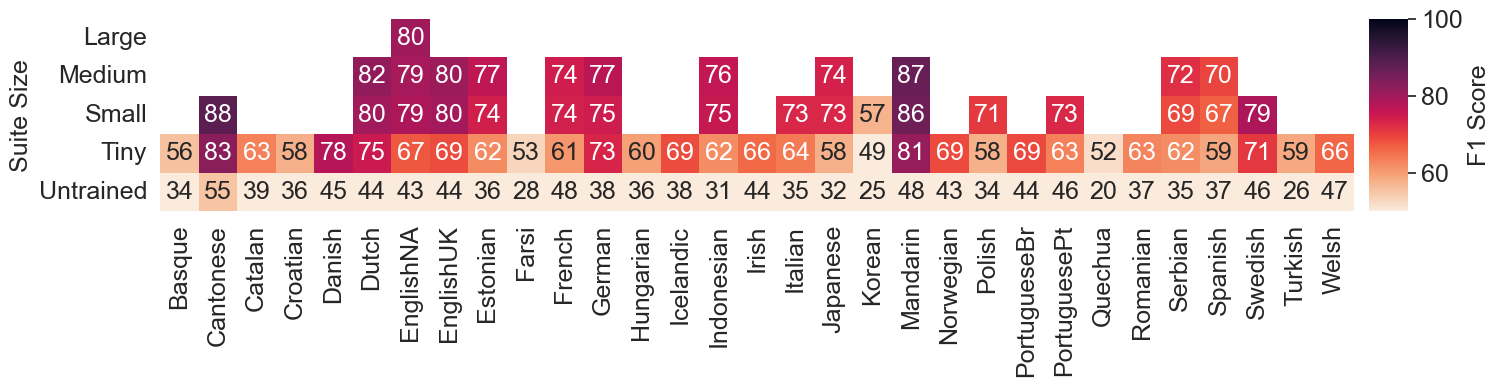
\includegraphics[width=\linewidth]{15Phonology/unsupervised.png}
    \caption{Boundary placement F1 scores achieved using the unsupervised segmentation strategies across models in each suite. For each score, we report the maximum across the 4 cues and 3 segmentation strategies. The Untrained row give the maximum scores achieved by each model in the Tiny suite before training.}
    \label{fig:15-unsupervised}
\end{figure}

% \begin{figure*}[t]
%     \centering
%     \includegraphics[width=\linewidth]{Figures/15Phonology/small_peak.png}
%     \caption{Boundary placement F1 scores achieved by each model in the Small suite using the \textbf{peak} segmentation strategy. The ``untrained'' column give the scores achieved by each model before training, averaged across all languages.}
%     \label{fig:15-peakscores}
% \end{figure*}

The results of the word boundary probe are presented in \cref{fig:15-probes} and the maximum boundary F1 scores of the unsupervised segmentation strategies are presented in \cref{fig:15-unsupervised}. The individual scores for each combination of language, suite size, boundary cue and segmentation strategy are provided in \cref{app:fullsegresults}. Significance between two probes is computed using McNemar's Test \citep{McNemar_1947} over the predicted word boundaries for the evaluation set, with a significance threshold of $p<0.05$. The same procedure is used when comparing the unsupervised methods.

Overall, both the word boundary probe and the unsupervised strategies successfully identify word boundaries --- all probes achieve accuracies significantly higher than the untrained baseline, as do the unsupervised strategies. The probe accuracies show that models implicitly track word boundaries in their contextual embeddings, suggesting that they are learning phonological rules to aid in next-phoneme prediction. The unsupervised segmentation results indicate that word boundaries can be extracted through prediction across many languages, corroborating previous statistical learning results about the role of distributional cues in language acquisition.

Below, these results are analysed in more detail.

\paragraph{180k words are sufficient for learning word boundaries.}
Across all languages, the accuracy of the word boundary probes increases from the Tiny suite to the Small suite (where models are trained on about \q{180}{\thousand} words, as seen in \cref{tab:15-suites}), but improvements are minimal for models in the larger suites. This also occurs with the unsupervised approach, despite receiving several orders of magnitude more training data and training with many more parameters. It is clear that \q{180}{\thousand} words is sufficient for a model to learn word-like units using this training framework.

%We conclude that 180k words and 3 layers are sufficient for a model to learn word-like units from unsegmented transcriptions.
% MAYBE ADD SOMETHING ABOUT PAST PAPERS LOOKING AT ORDER OF ACQUISITION


%In \cref{fig:15-sizes}, we plot the F1 score achieved by the models in each suite for each language, maximizing over the score achieved by each of the four cues. For most languages, there is a larger increase from Tiny to Small than from Small to Medium, but there are some exceptions. For instance, the largest performance increase for the German models occurs between the Small and Medium sizes. Meanwhile, the probe achieves the same accuracy of 86 for both. This indicates a discrepancy between the extent to which word boundaries can be extracted from contextual representations compared to being extracted from probability distributions produced by the model, which may become more stable with larger model sizes and training data availability.

% \begin{figure}[t]
%     \centering
%     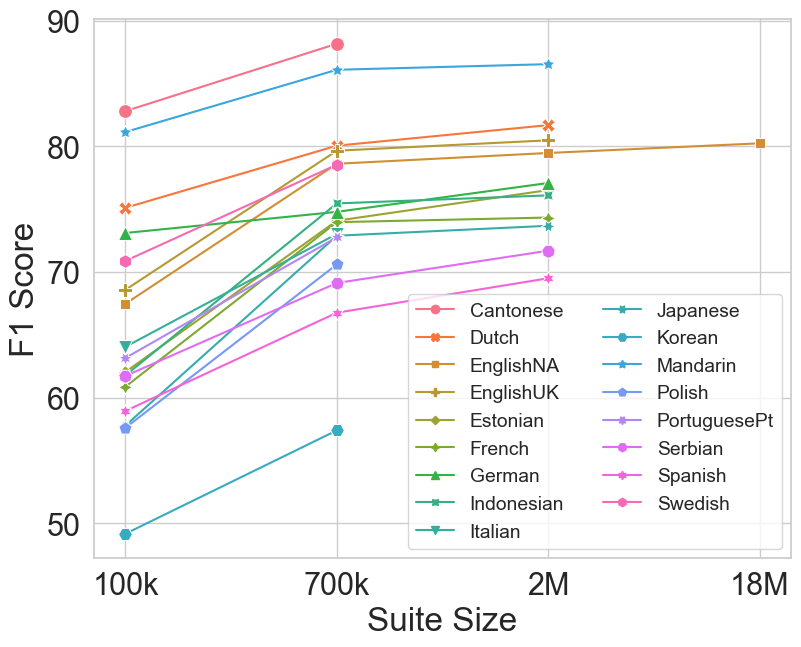
\includegraphics[width=\linewidth]{Figures/15Phonology/sizes.png}
%     \caption{Maximum boundary placement F1 scores achieved by each model across suite sizes. Only languages that appear in at least two suites are included.}
%     \label{fig:15-sizes}
% \end{figure}

% \begin{figure}[t]
%     \centering
%     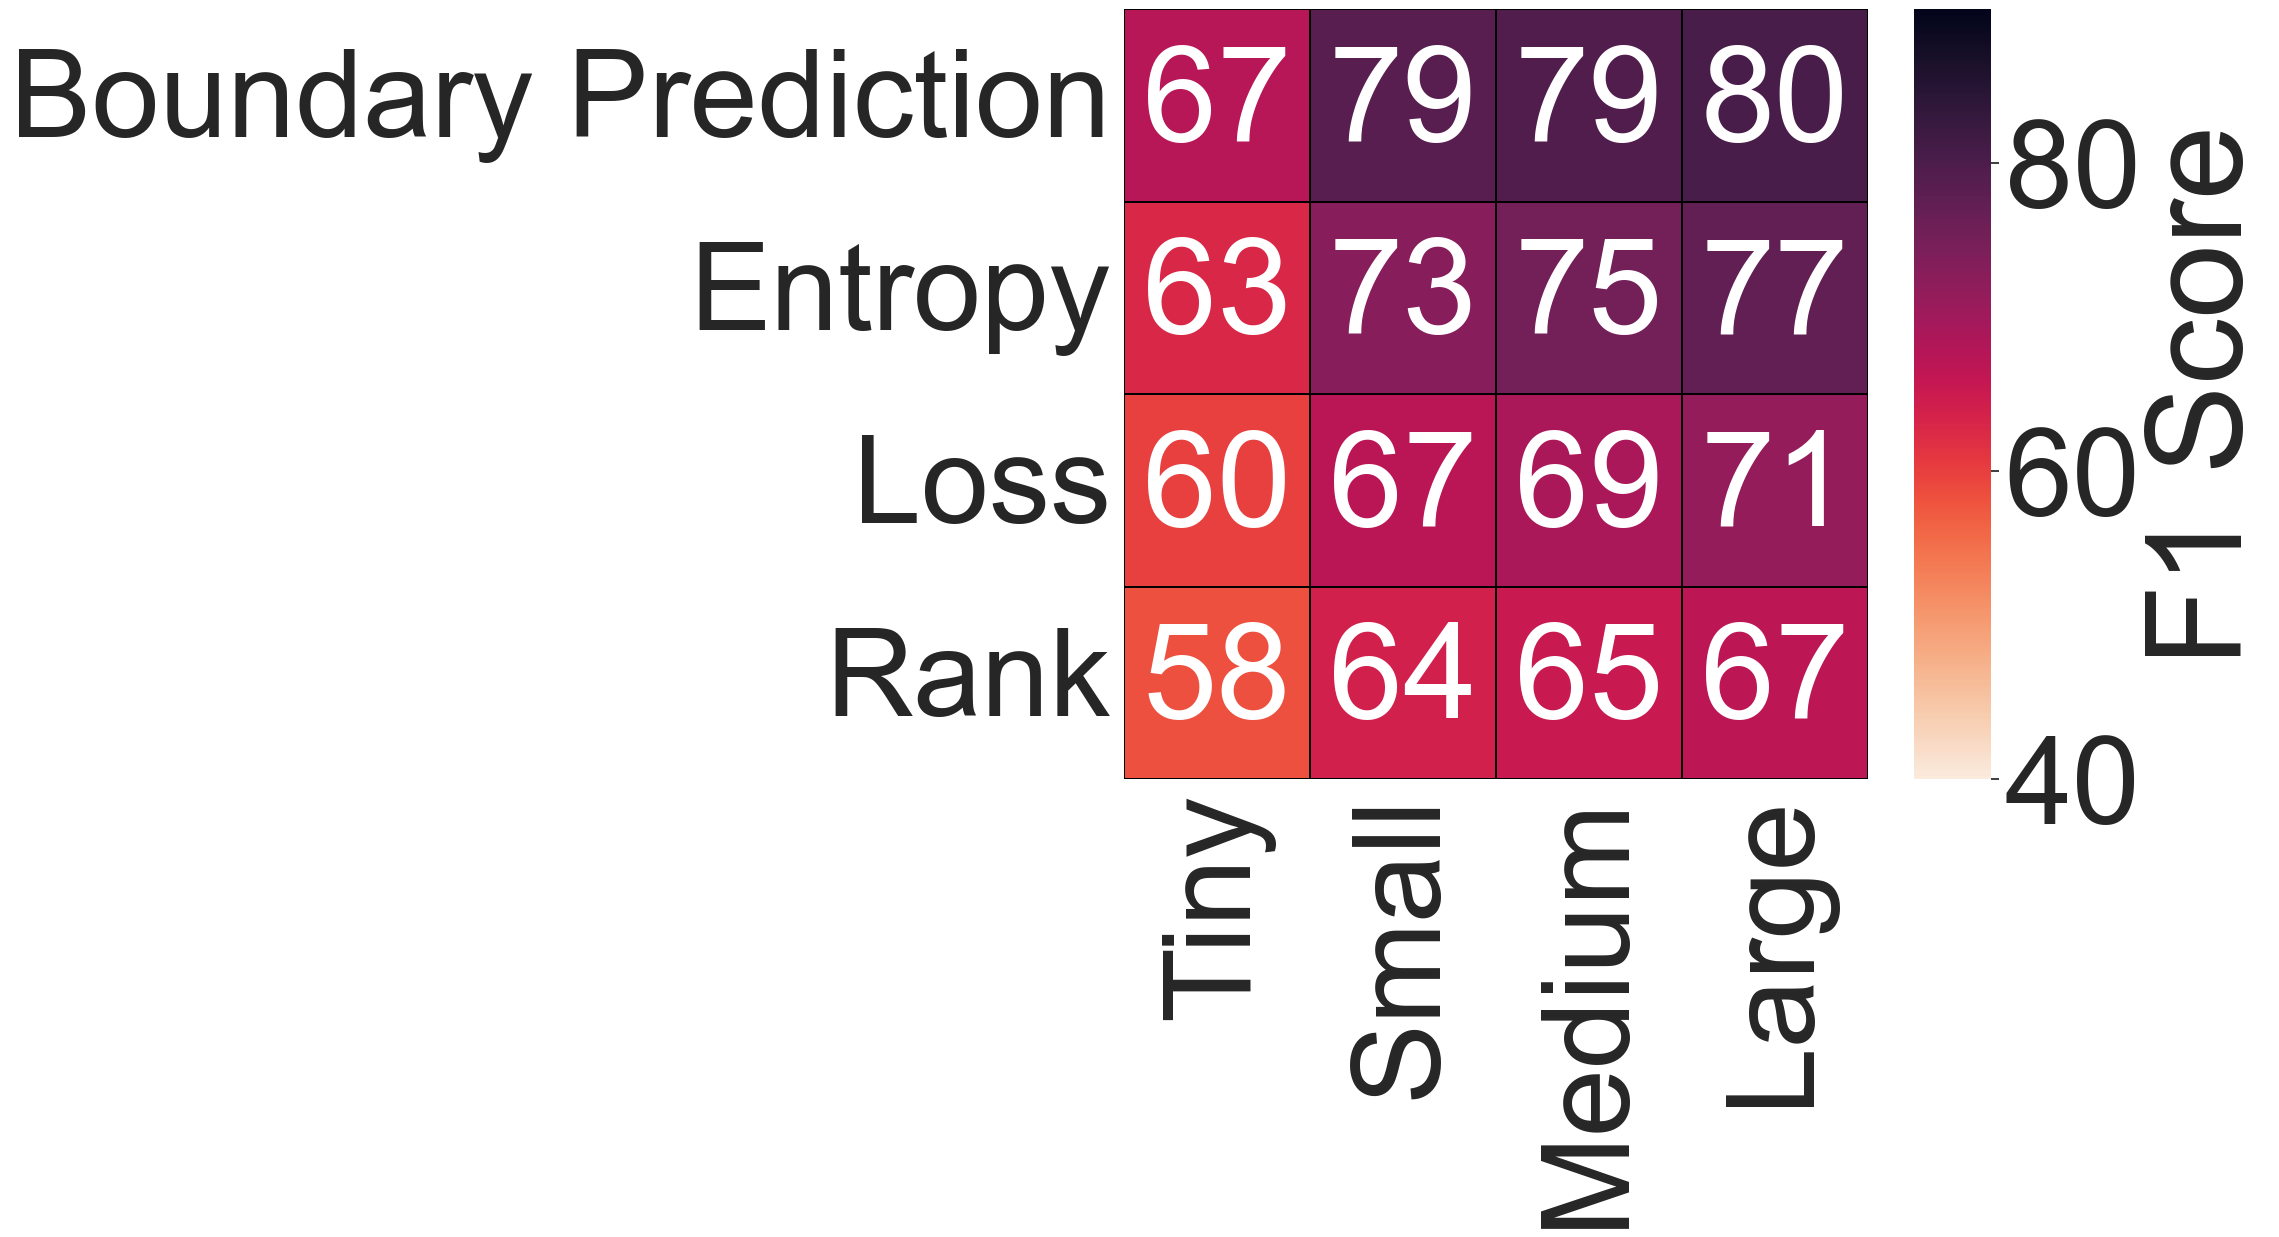
\includegraphics[width=\linewidth]{Figures/15Phonology/english_growth.png}
%     \caption{Boundary placement F1 scores achieved for the English model using the \textbf{peak} segmentation strategy across suite sizes.}
%     \label{fig:15-englishgrowth}
% \end{figure}

\paragraph{Utterance boundaries are better predictors of word boundaries than prediction-error.}
\Cref{fig:15-unsupervised} provides the maximum boundary F1 score achieved for each model in each suite across the four boundary cues and three segmentation strategies, for a total of 12 combinations. \Cref{tab:15-bestcues} summarises the cue and strategy combinations that achieved these scores. The UBP cue is the most effective in each suite, out-performing the three cues based on prediction-error, and the relative strategy out-performs the other two strategies. For reference, the best combination for each language is given in \cref{app:fullsegresults}. Generally, the best cue stays consistent across suites for a particular language (e.g. Entropy is the best cue for Italian), but this is not always the case, and the best strategy also varies. %[More analysis here]

\begin{table}[]
    \centering
    \small
    \begin{tabular}{lcccc}
    \toprule
    Cue \& Strategy & Tiny & Small & Medium & Large \\
    \midrule
    UBP (threshold) & 3 & 2 & 1 & - \\
    UBP (relative) & 3 & 6 & 4 & - \\
    UBP (peak) & 11 & 4 & 3 & 1 \\
    Entropy (threshold) & 1 & - & 1 & - \\
    Entropy (relative) & - & 4 & 2 & - \\
    Entropy (peak) & - & 1 & - & - \\
    %Loss (threshold) & - & - & - & - \\
    Surprisal (relative) & 9 & - & - & - \\
    %Loss (peak) & - & - & - & - \\
    %Rank (threshold) & - & - & - & - \\
    Rank (relative) & 3 & - & - & - \\
    Rank (peak) & 1 & - & - & - \\
    \bottomrule
    \end{tabular}
\caption{Counts of the word boundary cues and segmentation strategies that achieved the highest F1 scores in each suite.}
\label{tab:15-bestcues}
\end{table}

%We compare four cues for our unsupervised word segmentation strategy, one based on utterance boundary probability and three based on prediction-error. Examining the Small suite peak segmentation results in \cref{fig:15-peakscores}, we find that the Boundary Prediction cue achieves the highest F1 score for 13 of the 17 languages. Of the three prediction-error cues, Entropy scores higher than Loss or Rank for 15 of the 17 languages.

\paragraph{The peak segmentation strategy fails to capture subsequent boundaries.}
\Cref{fig:15-qualitative} compares the output of the peak strategy for all four cues, operating over utterances from the EnglishNA portion of \ipachildes. There seem to be two failure modes for this strategy. The first is that since two peaks cannot directly follow one another, subsequent boundaries cannot both be successfully placed. In this example, the \ttipa{h} in ``help'' is incorrectly placed by all four cues. A second failure mode is that the relative size of peaks is not considered; three cues incorrectly place a boundary within the word ``fingers'' due to a very small peak at \ttipa{\textschwa}. The threshold and relative segmentation strategies address both of these issues but for English the peak strategy is still best overall.

% SEE \cref{app:15-qualitative})

\begin{figure*}
    \centering
    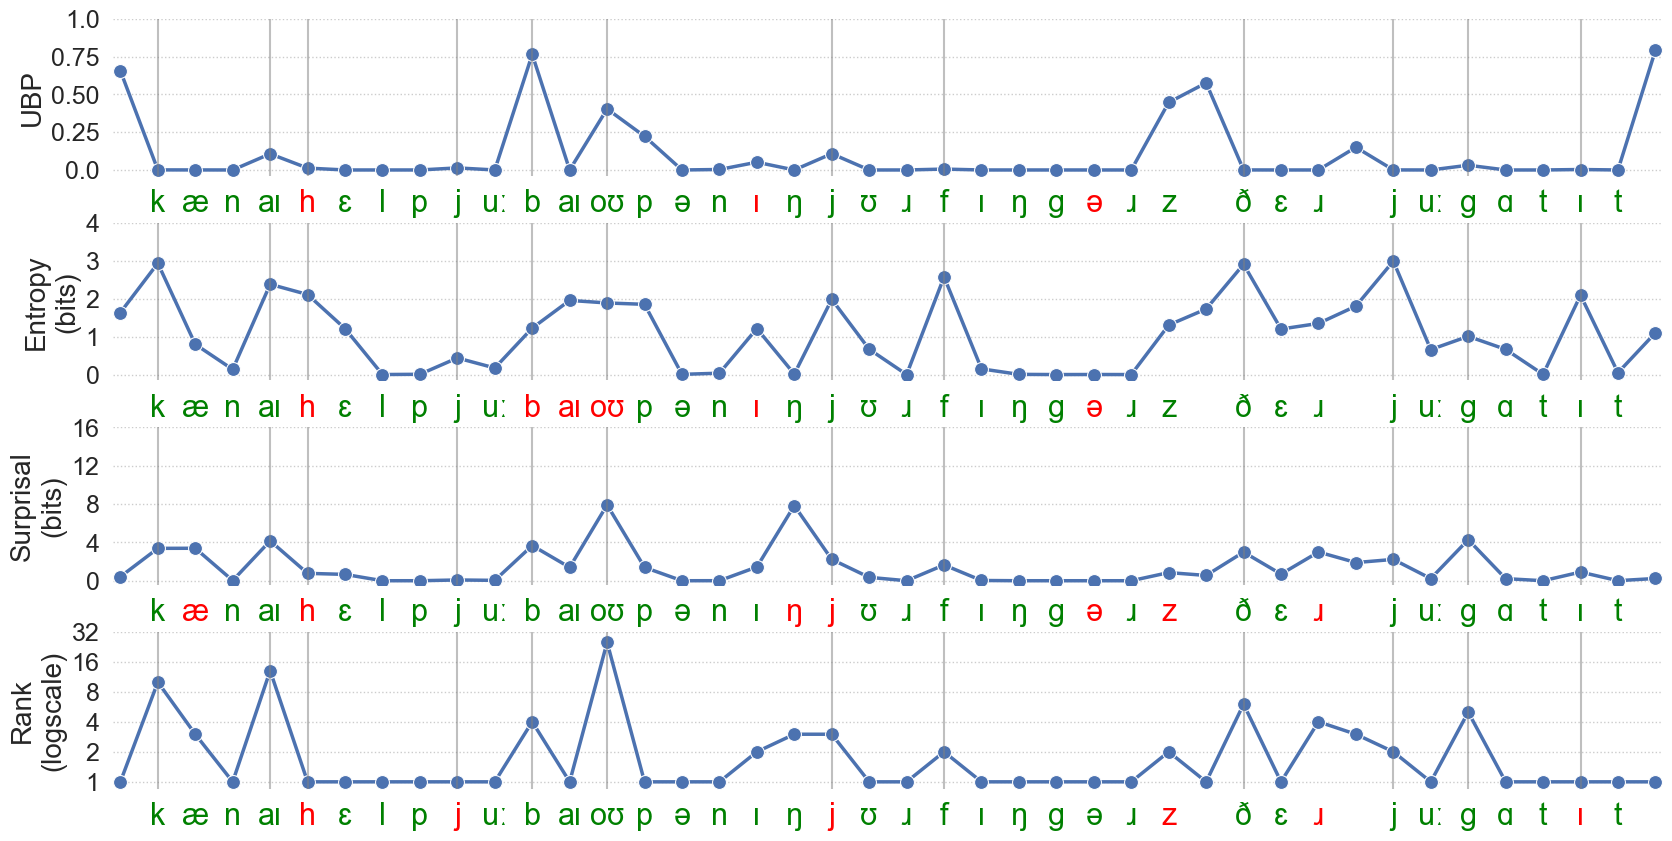
\includegraphics[width=\linewidth]{Figures/15Phonology/qualitative.png}
    \caption{Per-phoneme boundary probability, entropy, surprisal and rank assigned by the Medium English model for the sequence of utterances ``can I help you by opening your fingers'', ``there'', ``you got it''. Spaces indicate utterance boundaries, vertical lines indicate gold word boundaries and phonemes are marked as green if they are correctly identified as word boundaries using the \textbf{peak} strategy or if they follow an utterance boundary (red otherwise).}
    \label{fig:15-qualitative}
\end{figure*}

% \emph{Qualitative evaluation of the English model is given in \cref{fig:15-qualitative}. First, we note one of the failure cases for the peak segmentation strategy. Since by definition one peak can't follow another, the \ttipa{h} in ``help'' cannot be correctly identified as a word boundary for any measure after preceding \ttipa{aI} is correctly identified.}

% \emph{Considering the relatively longer words ``opening'' and ``fingers'', we see that when segmenting with the Boundary Probability or Entropy cue, the `incorrect' boundary split the words into possible morphemes, ``open''+``ing'' and ``fing'' + ``ers''. This last segmentation is barely visible on the plot and this segmentation probably should not happen given that `e` appears 99.9\% of the time after `fing` in the training dataset, but since the strategy only captures relative certainty, we incorrectly place a word boundary. }

\begin{figure}[t]
\centering
\begin{subfigure}{0.95\linewidth}
    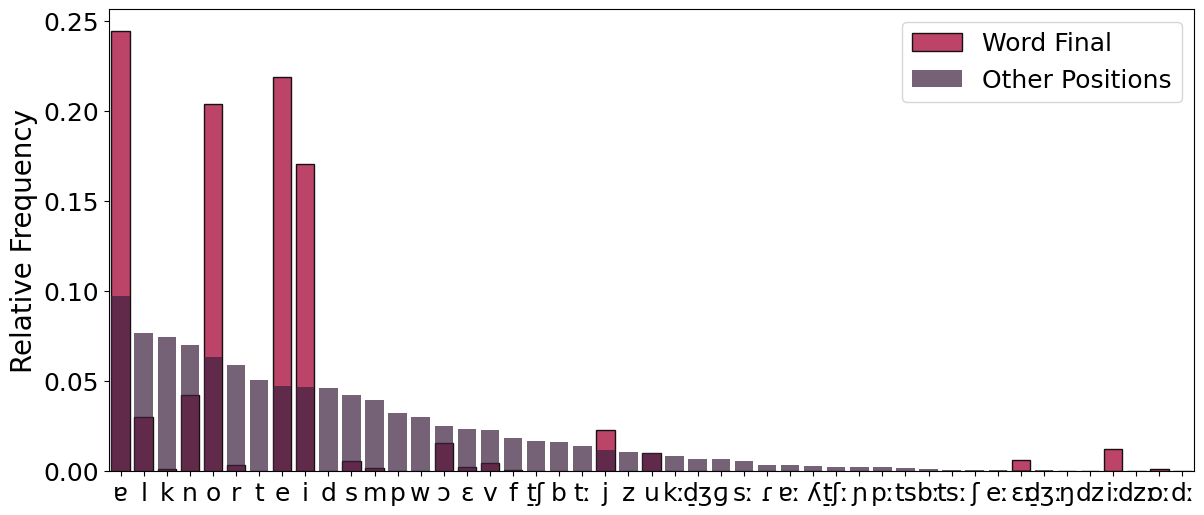
\includegraphics[width=\linewidth]{Figures/15Phonology/italian.png}
\end{subfigure}
\hfill
\begin{subfigure}{0.95\linewidth}
    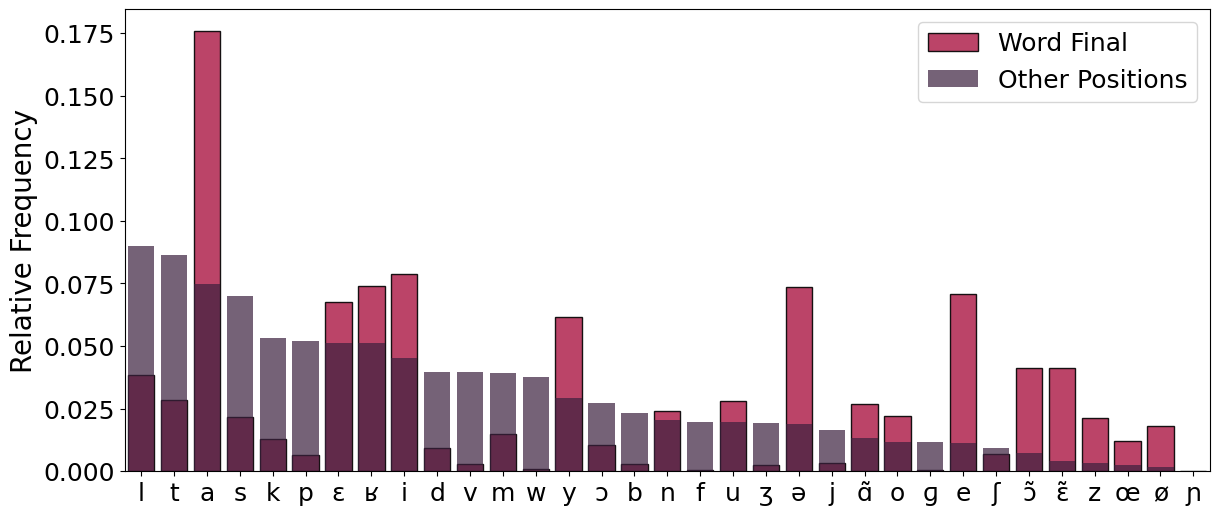
\includegraphics[width=\linewidth]{Figures/15Phonology/french.png}
\end{subfigure}
\hfill
\caption{Relative frequencies of phonemes appearing in word-final positions and all other positions for Italian (top) and French (bottom).}
\label{fig:15-frequencies}
\end{figure}

%the same number of word-final embeddings, labelled as boundary positions, as the number of non-word-final embeddings
%they must identify word-final contextual embeddings, with all other positions labelled as non-boundary
%where the the number of word-final embeddings used to train the probe is equal to the number non-word-final embeddings

\paragraph{Italian has a strong prior for learning word boundaries.}
\citet{hahn-baroni-2019-tabula} claim that since the probes are trained on balanced examples,
chance accuracy should be 50\%. However, probes trained on completely untrained models (see \cref{fig:15-probes}) achieve accuracies ranging from 51\% for French up to 68\% for Italian. This is because the balancing procedure does not account for the fact that phonemes have different probability distributions depending on their position within words. For example, \cref{fig:15-frequencies} shows that at the end of Italian words, a small number of phonemes have particularly high frequencies (the vowels \ttipa{\textturna, o, e} and \ttipa{i} end 84\% of words) whereas the distribution of French word-final phonemes is not as skewed. This skewed distribution provides a useful prior for the Italian probe, which can achieve high accuracies by relying on these phoneme frequencies (the only signal available when using embeddings from an unsupervised model). To measure the relative benefit of each prior, the \textbf{normalised entropy} of the word-final phoneme distributions in each language can be computed, 

$$H_\mathrm{norm}=\frac{H(P)}{H_\mathrm{max}} = \frac{\sum_{i=1}^np_i\log_ip_i}{log_2(n)},$$ 
which ranges from \integer{0} (deterministic distribution) to \integer{1} (uniform distribution). Not only do Italian and French have the lowest and highest normalised entropies with \integer{0.51} and \integer{0.84}, respectively, but in general, this normalised entropy has a high negative correlation with probe accuracy for the untrained models (Pearson $\rho = -0.69$). This correlation is still present for the Tiny suite (Pearson $\rho = -0.52$) but is not significant for the Small and Medium suites, indicating that although the word-final phoneme distribution prior is useful, the embeddings do still encode information about word boundaries that the probes can detect.

%This finding indicates that the word segmentation task may be inherently easier for some languages than others when relying solely on distributional information.  he Italian probe does perform the best in each suite, however still significantly improves over its baseline, indicating that the model is still learning to track boundaries. 

%We can measure how skewed the word-final distributions are by computing the entropy of the word-final phoneme distributions and normalizing it (dividing by $log(n)$ where $n$ is the number of phonemes for that language). This gives a score between 0 and 1 for each language where 0 indicates a deterministic distribution and 1 indicates a uniform distribution. We find that not only do Italian and French have the lowest and highest relative entropies with 0.51 and 0.84, respectively, but in general, this relative entropy has a high negative correlation with probe accuracy for the untrained models (spearman -0.70). This correlation drops to -0.48, -0.47 and -0.09 for the Tiny, Small and Medium suite results, the last two of which are not significant, presumably because as the models grow they learn more sophisticated distributional patterns that the probe can use to its advantage.
%suggesting that once the models reach a certain size they are learning distributional patterns more sophisticated than simple phoneme frequency. 


\paragraph{Word length is a confounding factor for unsupervised segmentation.}
Just as with the probes, using the unsupervised methods on untrained models can reveal confounding factors, as shown in \cref{fig:15-unsupervised}. The F1 scores for the untrained models range from \integer{20} for Quechua up to \integer{55} for Cantonese. For 25 of the 31 languages, this score comes from the UBP cue with the relative strategy; since the probability of an utterance boundary from an untrained model will randomly vary over the phoneme sequence, boundary placement using the relative strategy essentially places boundaries randomly, which can still yield relatively high F1 scores if words are short. This seems to be the case here; Quechua has the highest average word length in \ipachildes and Cantonese has the lowest, with \integer{6.2} and \integer{2.4} phonemes per word, respectively. Generally, word length has a high negative correlation with the \fscores with Pearson $\rho = -0.94, -0.71, -0.79, -0.42$ for the Untrained, Tiny, Small and Medium suites, respectively (although the final correlation is not significant). 

This confounding factor means that word segmentation scores cannot be easily compared between languages, only scores for each language across suite sizes. Compared to the untrained models, the unsupervised word segmentation strategy still achieves significantly higher \fscores for every language, demonstrating that distributional information is a useful cue for bootstrapping a lexicon. 

% \emph{Past computational models of word segmentation have mostly focused on English. In their multilingual study, \citet{goriely2023word} found that English achieved one of the highest boundary F1 scores. Here, English does perform relatively well for unsupervised segmentation but not necessarily for the probe, where for the Tiny suite English is on the lower end. On the other hand, unsupervised segmentation with the Korean model...}

\section{Experiment: Probing for distinctive phonological features}\label{sec:15-featureprobing}

In the previous experiment, linear probes were used to explore whether the contextual embeddings of phonemes implicitly encode information about word boundaries, despite no word boundaries being presented to the model during training. Here, linear probes are used to explore whether \defn{distinctive phonological features} are also encoded in these representations. Distinctive features are the basic units used in phonology to represent how phonemes differ from each other in terms of articulatory or acoustic properties. Since phoneme LMs are only exposed to distributional information, probing them for distinctive features may reveal whether these features play a role in distributional phonology. 

\setlength{\tabcolsep}{1pt}
\begin{table}[t]
    \small
    \centering
    \begin{tabular}{*{38}{c}}
     \rotatebox{90}{advanced tongue root} 
     & \rotatebox{90}{anterior} 
     & \rotatebox{90}{approximant} 
     & \rotatebox{90}{back} 
     & \rotatebox{90}{click} 
     & \rotatebox{90}{consonantal} 
     & \rotatebox{90}{constricted glottis} 
     & \rotatebox{90}{continuant} 
     & \rotatebox{90}{coronal} 
     & \rotatebox{90}{delayed release} 
     & \rotatebox{90}{distributed} 
     & \rotatebox{90}{dorsal} 
     & \rotatebox{90}{epilaryngeal source} 
     & \rotatebox{90}{fortis} 
     & \rotatebox{90}{front} 
     & \rotatebox{90}{high} 
     & \rotatebox{90}{labial} 
     & \rotatebox{90}{labiodental} 
     & \rotatebox{90}{lateral} 
     & \rotatebox{90}{long} 
     & \rotatebox{90}{low} 
     & \rotatebox{90}{lowered larynx implosive} 
     & \rotatebox{90}{nasal} 
     & \rotatebox{90}{periodic glottal source} 
     & \rotatebox{90}{raised larynx ejective} 
     & \rotatebox{90}{retracted tongue root} 
     & \rotatebox{90}{round} 
     & \rotatebox{90}{short} 
     & \rotatebox{90}{sonorant} 
     & \rotatebox{90}{spread glottis} 
     & \rotatebox{90}{stress} 
     & \rotatebox{90}{strident} 
     & \rotatebox{90}{syllabic} 
     & \rotatebox{90}{tap} 
     & \rotatebox{90}{tense} 
     & \rotatebox{90}{tone} 
     & \rotatebox{90}{trill} \\
    0 & 0 & -- & 0 & -- & + & -- & -- & -- & 0 & 0 & -- & -- & -- & 0 & 0 & + & -- & -- & -- & 0 & -- & + & + & -- & 0 & -- & -- & + & -- & -- & 0 & -- & -- & 0 & 0 & -- \\
    \end{tabular}
    \caption{Distinctive phonological features listed in \phoible for the phoneme \textipa{m}.}
    \end{table}
    \label{tab:15-features}
\setlength{\tabcolsep}{6pt}

There are several schemes for distinctive features, many of which use binary properties. Broadly, \emph{major class} features separate broad categories like vowels or consonants, \emph{manner features} express how air flows during articulation, \emph{place features} describe where in the vocal tract sound is articulated, \emph{laryngeal features} express laryngeal activity and \emph{vowel features} describe how vowels are articulated. For example, the \texttt{consonantal} feature is a major class feature which indicates an audible constriction of the vocal tract, separating obstruents, nasals, liquids, and trills from vowels, glides and laryngeal segments \citep{gussenhoven2017understanding}.

The \phoible database uses a scheme with 37 features, based on \citet{hayes2011introductory} and \citet{moisik2011whole}. For a given phoneme, \ex{+} indicates that the feature is present, \ex{-} indicates that it is not present and \ex{0} indicates that the feature is not applicable (for instance, vowel features are not applicable to consonants). An example of the set of features listed for the consonant \textipa{m} is shown in \cref{tab:15-features}. Past work has explored whether these features could be used as linguistically-motivated embeddings for phonemes (a 37-dimensional vector) but found that such embeddings perform worse than data-driven learned embeddings \citep{sofroniev-coltekin-2018-phonetic}.

Since \gpp uses folding maps to ensure that output phonemes maintain a correspondence with \phoible inventories, and \gpp was used to create \ipachildes (as described in \cref{chapter:resources}), these features can easily be accessed for each phoneme in \ipachildes, supporting the implementation of these probes.

\subsection{Related work}

Past work has explored whether distinctive features are encoded in phoneme embeddings. For instance, \citet{kolachina-magyar-2019-phone} learn phoneme embeddings for artificially constructed languages using \myemph{word2vec}, finding that phonological relationships are encoded. Similarly, \citet{silfverberg2018sound} explore whether distinctive features are encoded directionally in phoneme embeddings for Finnish, Turkish and Spanish using phoneme embeddings learned with \myemph{word2vec} or an RNN encoder-decoder trained on a morphological inflection task. Most recently, \citet{astrach2025probing} train transformer-based encoder-decoder models on the morphological inflection task for seven languages, using data from the SIGMORPHON shared task \citep{cotterell-etal-2017-conll} converted to phonemes using \myemph{epitran}. They probe both the embedding layer and the contextual embeddings for distinctive features, finding that the degree to which distinctive features are encoded depends on the feature's importance for the morphology and phonology of the language the model is trained for. All three of these examples use models that learn encodings on individual words. Here, representations learned from phoneme LMs trained on naturalistic child-directed speech are probed for phonological features, and these are evaluated on 11 languages.

\subsection{Distinctive feature probe}

Phonological feature probes are implemented for each of the 11 phoneme LMs in the Medium suite (see \cref{sec:15-suite}). The set of unique phonemes for each language is extracted from the corresponding \phoible entry for that language (as listed in \cref{tab:13-ipa-childes-sections}). For some languages, certain features do not distinguish many phonemes. For example, in the English \phoible inventory, only \textipa{h} has the \texttt{+spreadGlottis} feature, so a probe for \texttt{spreadGlottis} could succeed just by identifying embeddings for \texttt{h}. For this experiment, the only features used are those for which, in all 11 languages, there are at least 4 phonemes that exhibit the feature and 4 that do not. 

For each feature $f$, a linear probe $p_f$ is trained to predict that feature from the contextual embeddings $c(x)$ of phonemes. Each probe is trained with an equal number of positive and negative examples and is evaluated using leave-one-group-out cross-validation (i.e for each phoneme $x$ in the phoneme inventory $V$, the probe is trained on the contextual embeddings of all other phonemes $\{c(y) | y\in V \setminus \{x\}\}$, then evaluated by predicting the feature from contextual embeddings of the left-out phoneme $p_f(c(x))$, and the final score is a macro-average across all phonemes $x\in V$). As with the word boundary probes above, accuracy is used to report the performance of each probe.

\subsection{Results}

\begin{figure}[t]
    \centering
    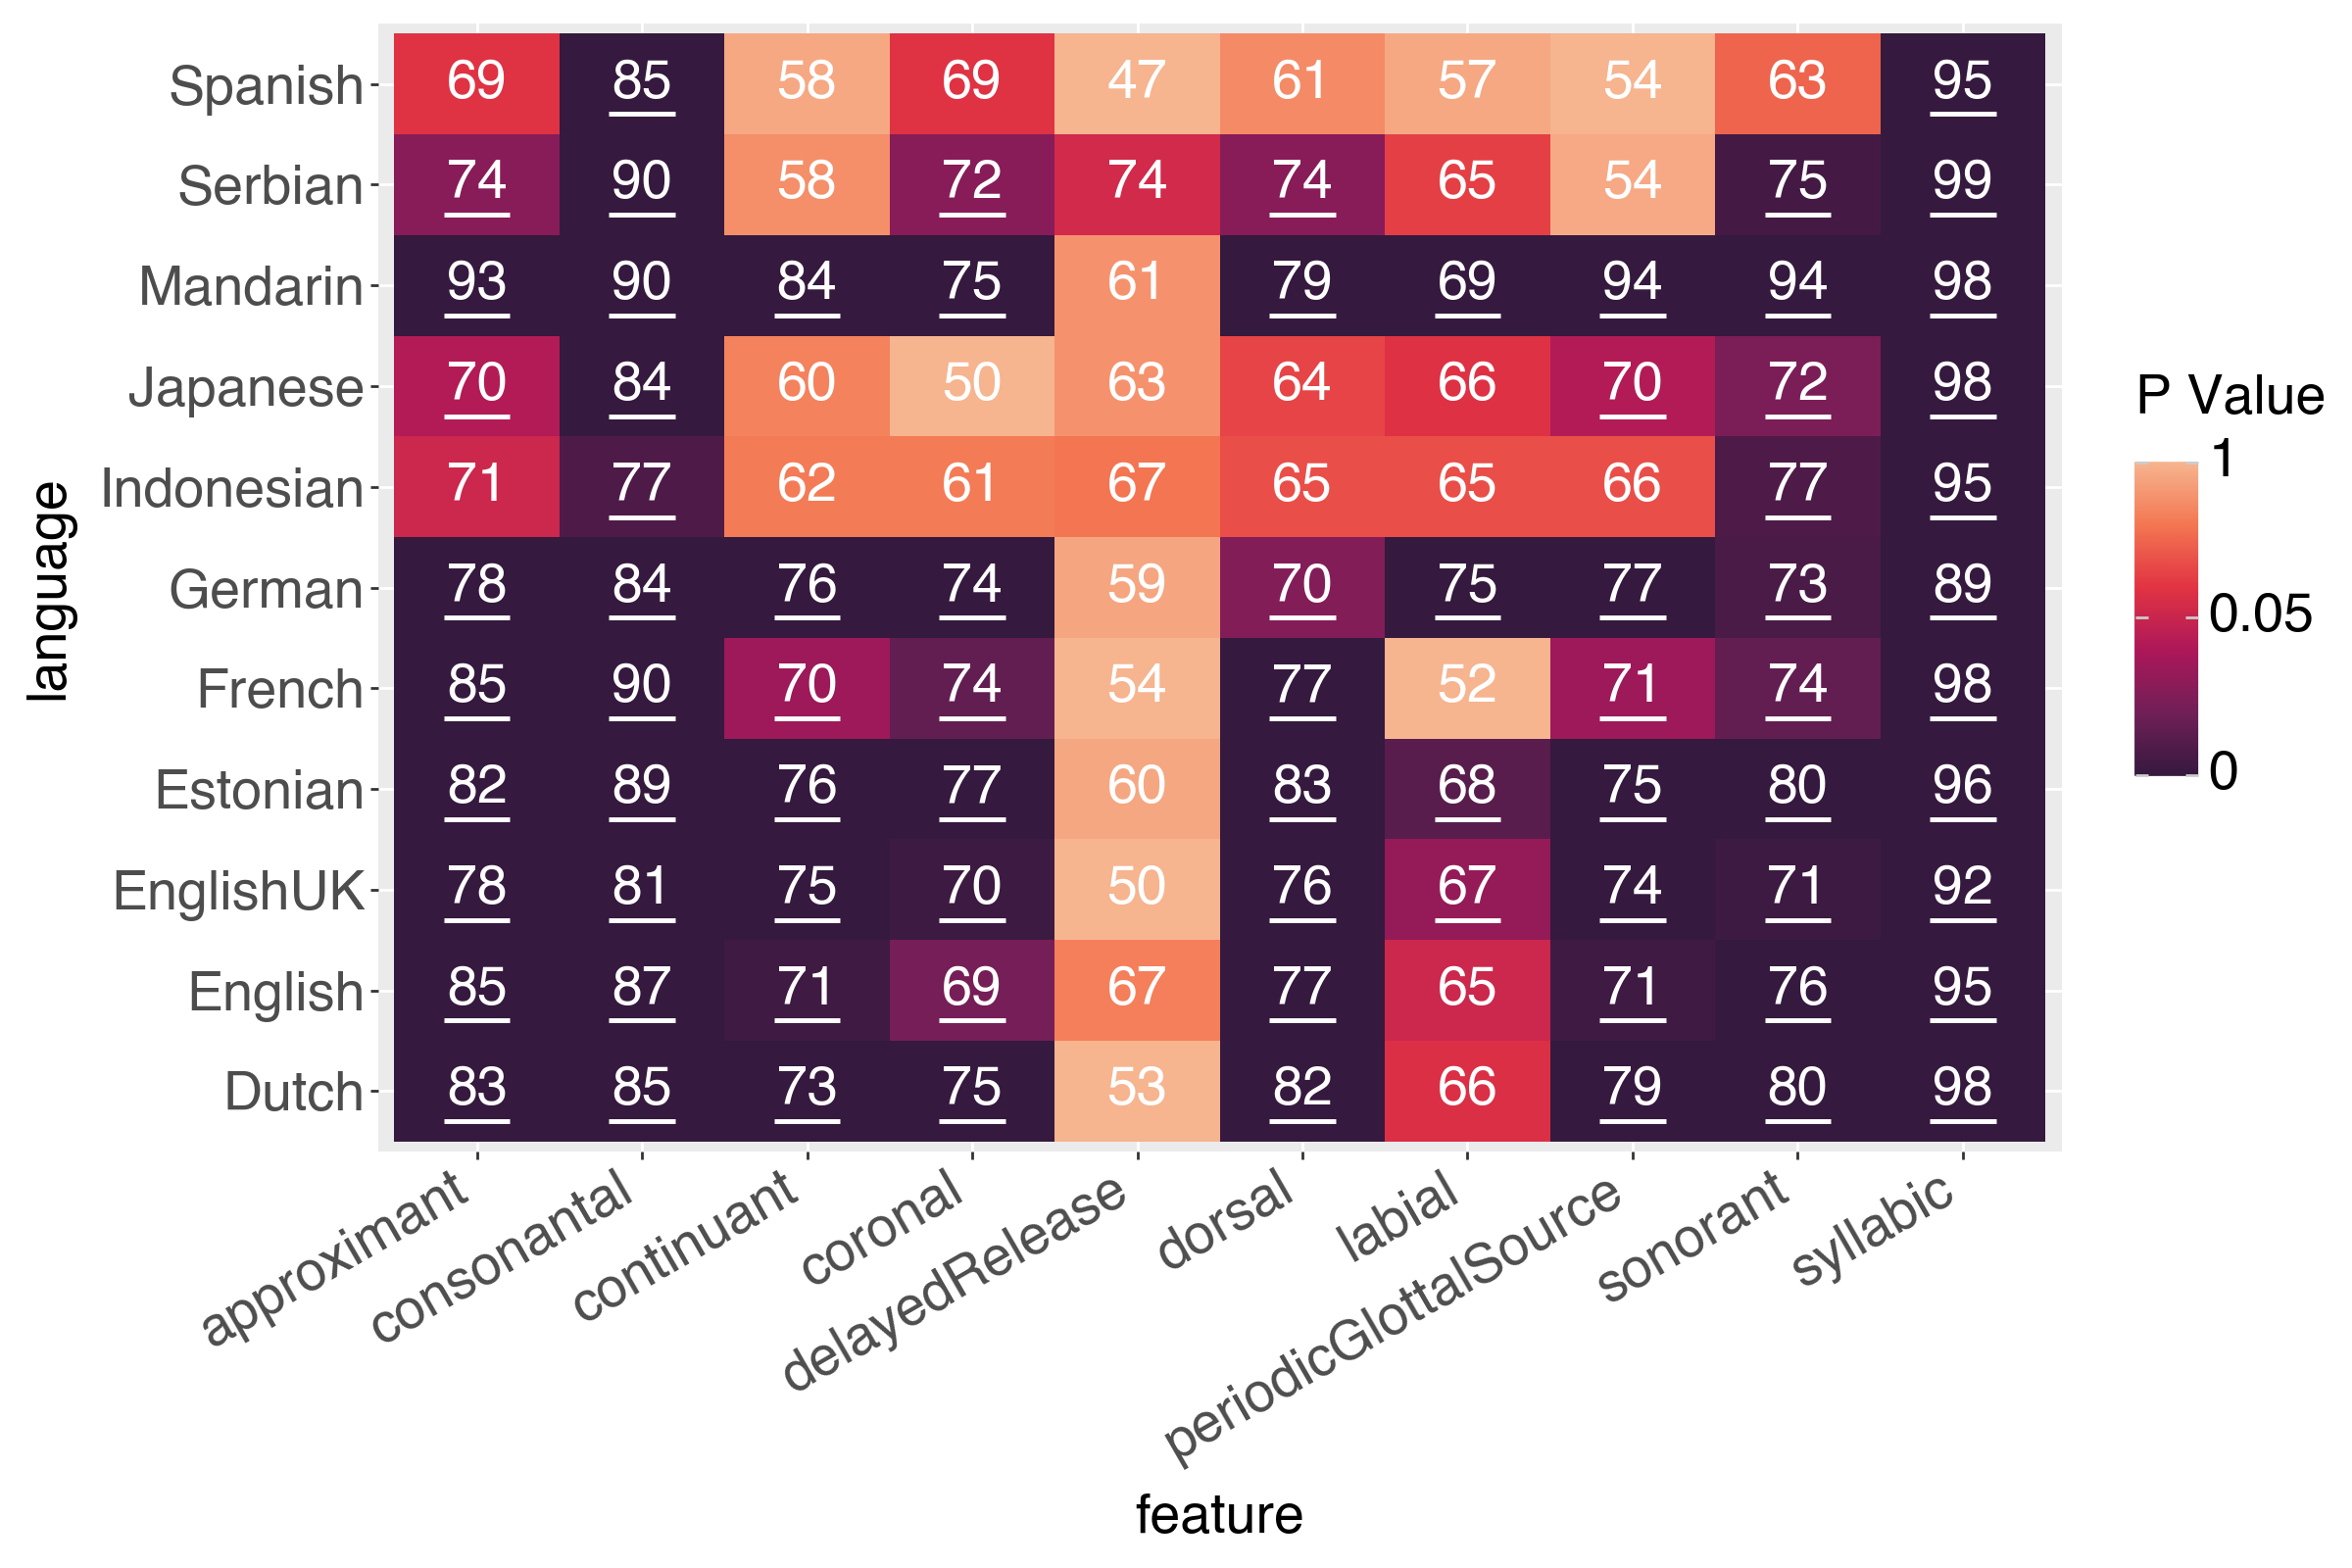
\includegraphics[width=0.99\linewidth]{15Phonology/features.png}
    \caption{Accuracy of the phonological distinctive feature probe across 11 languages in \ipachildes and 9 distinctive features from \phoible.}
    \label{fig:features}
\end{figure}

\begin{figure}[t]
    \centering
    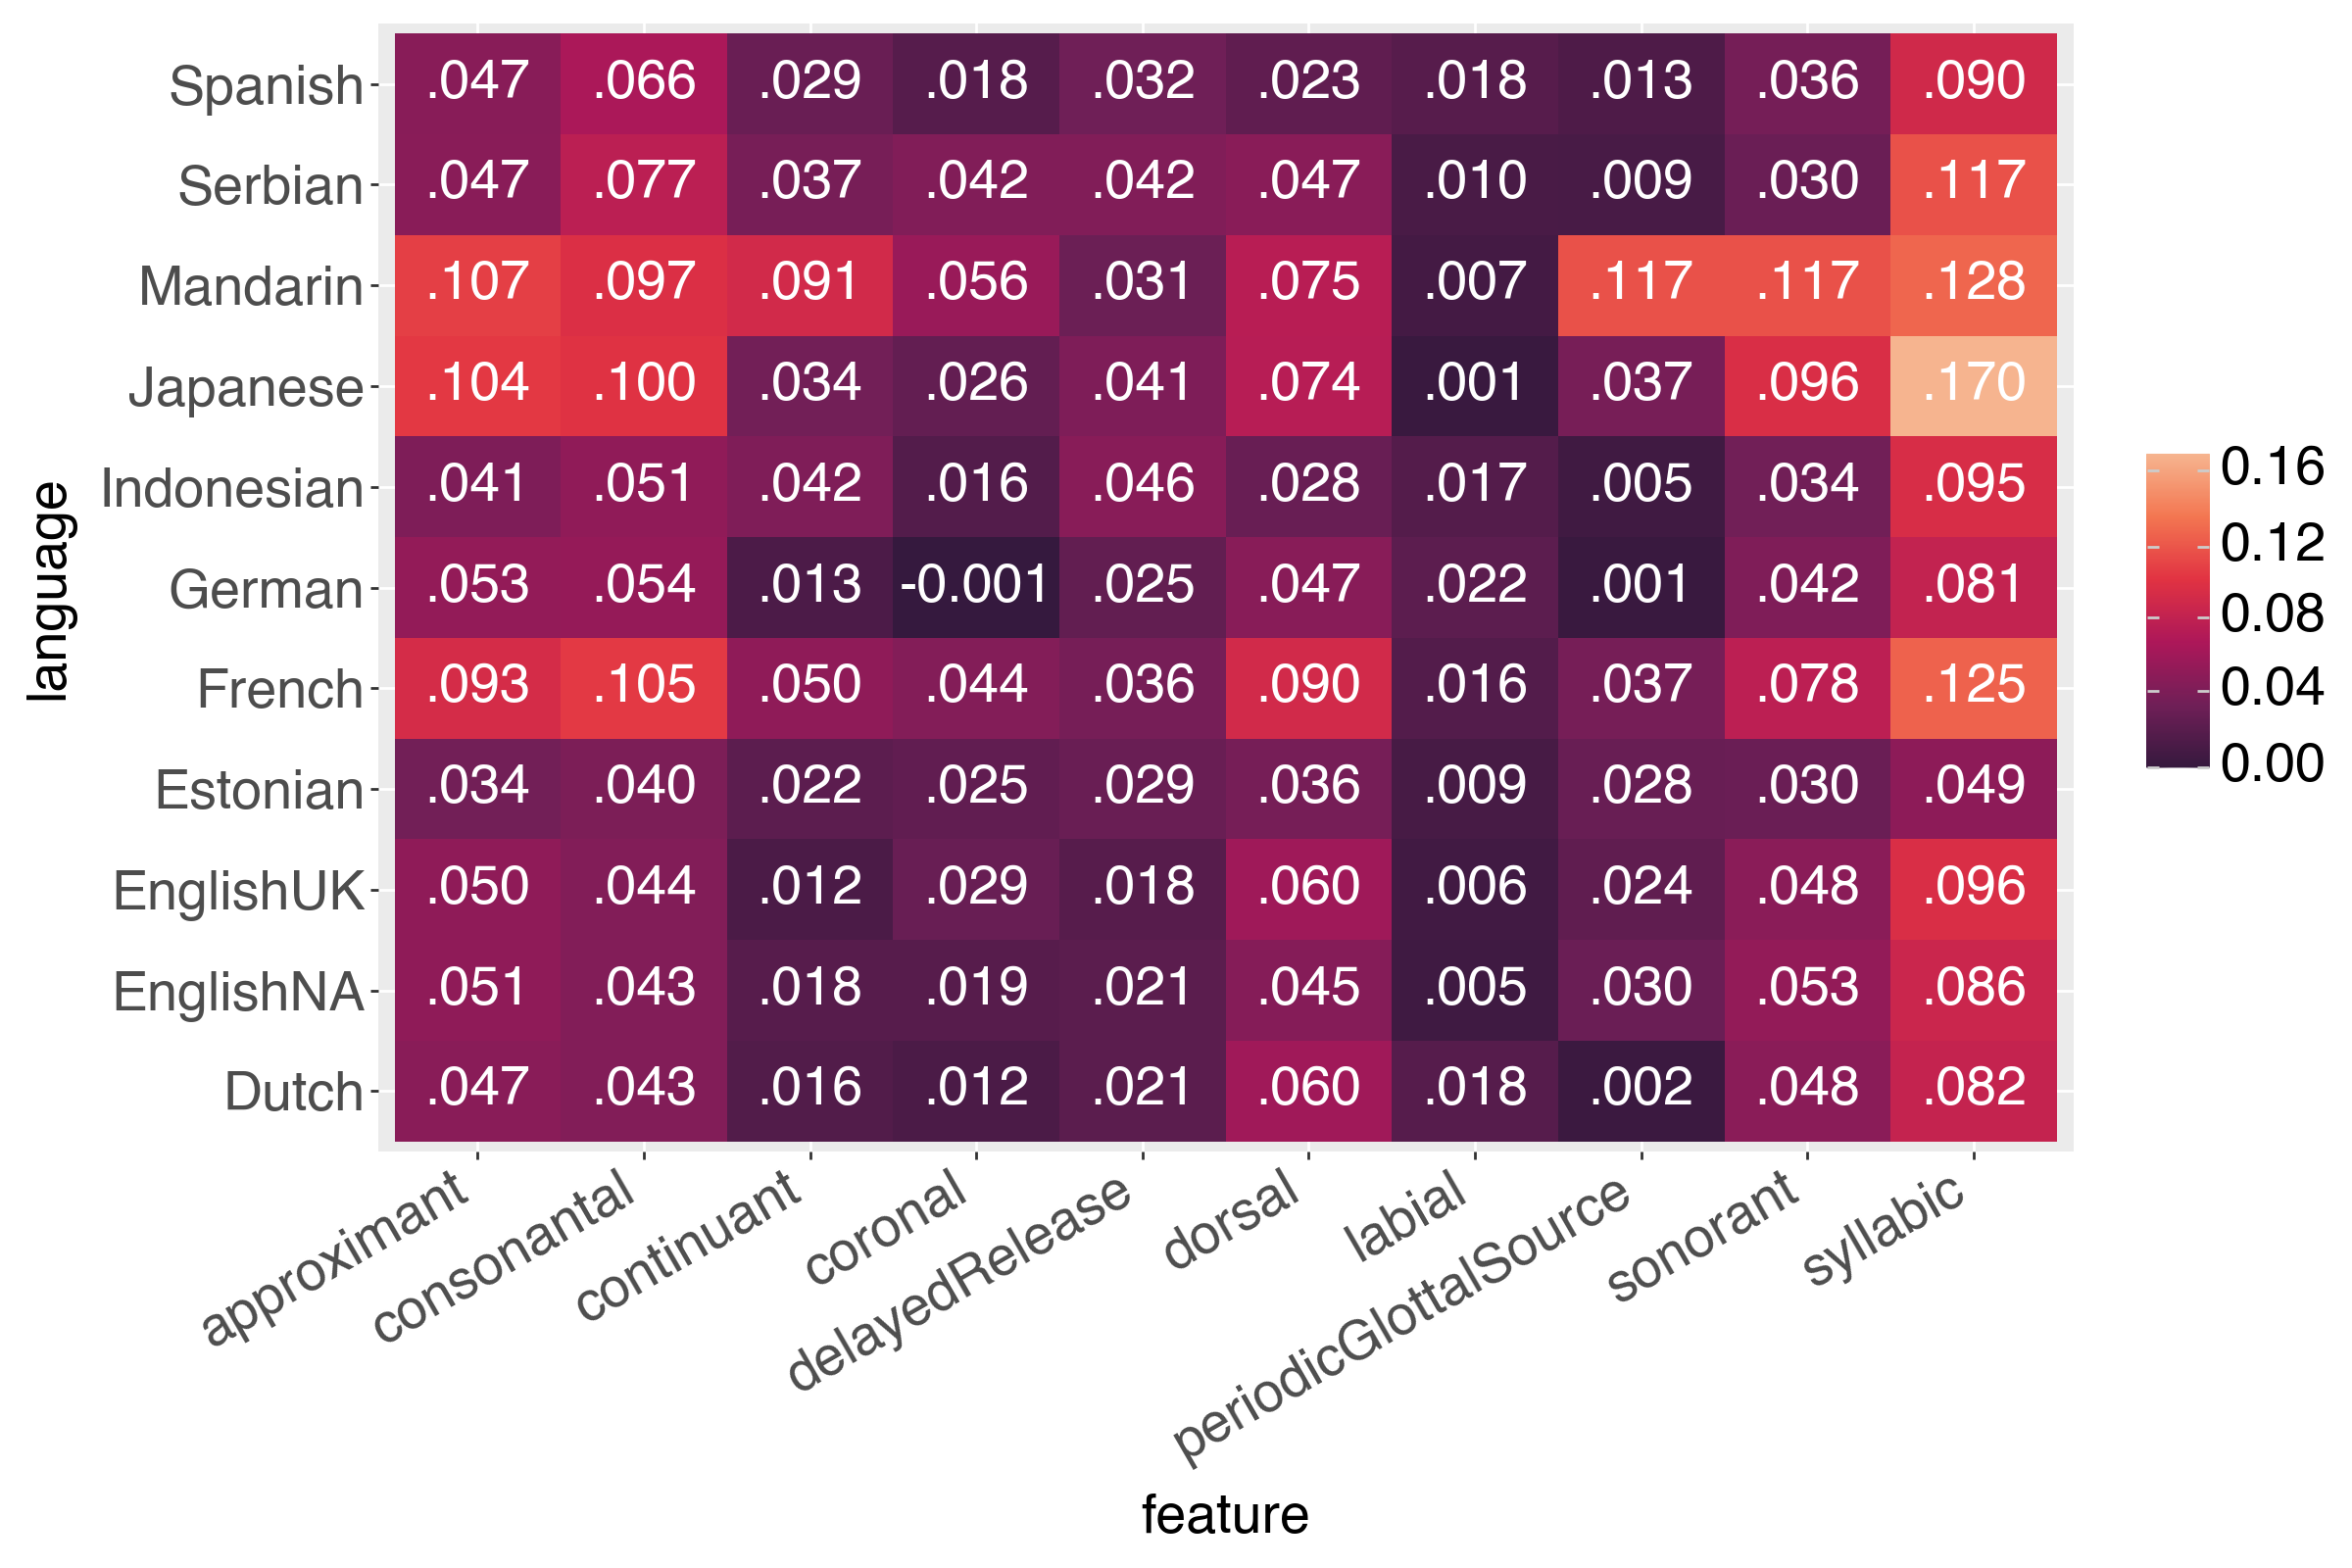
\includegraphics[width=0.99\linewidth]{15Phonology/silhouette.png}
    \caption{Average silhouette scores when using each distinctive feature to cluster contextual embeddings of the phonemes in each language.}
    \label{fig:silhouette}
\end{figure}

\begin{figure}[t]
    \centering
    \begin{subfigure}{0.49\textwidth}
        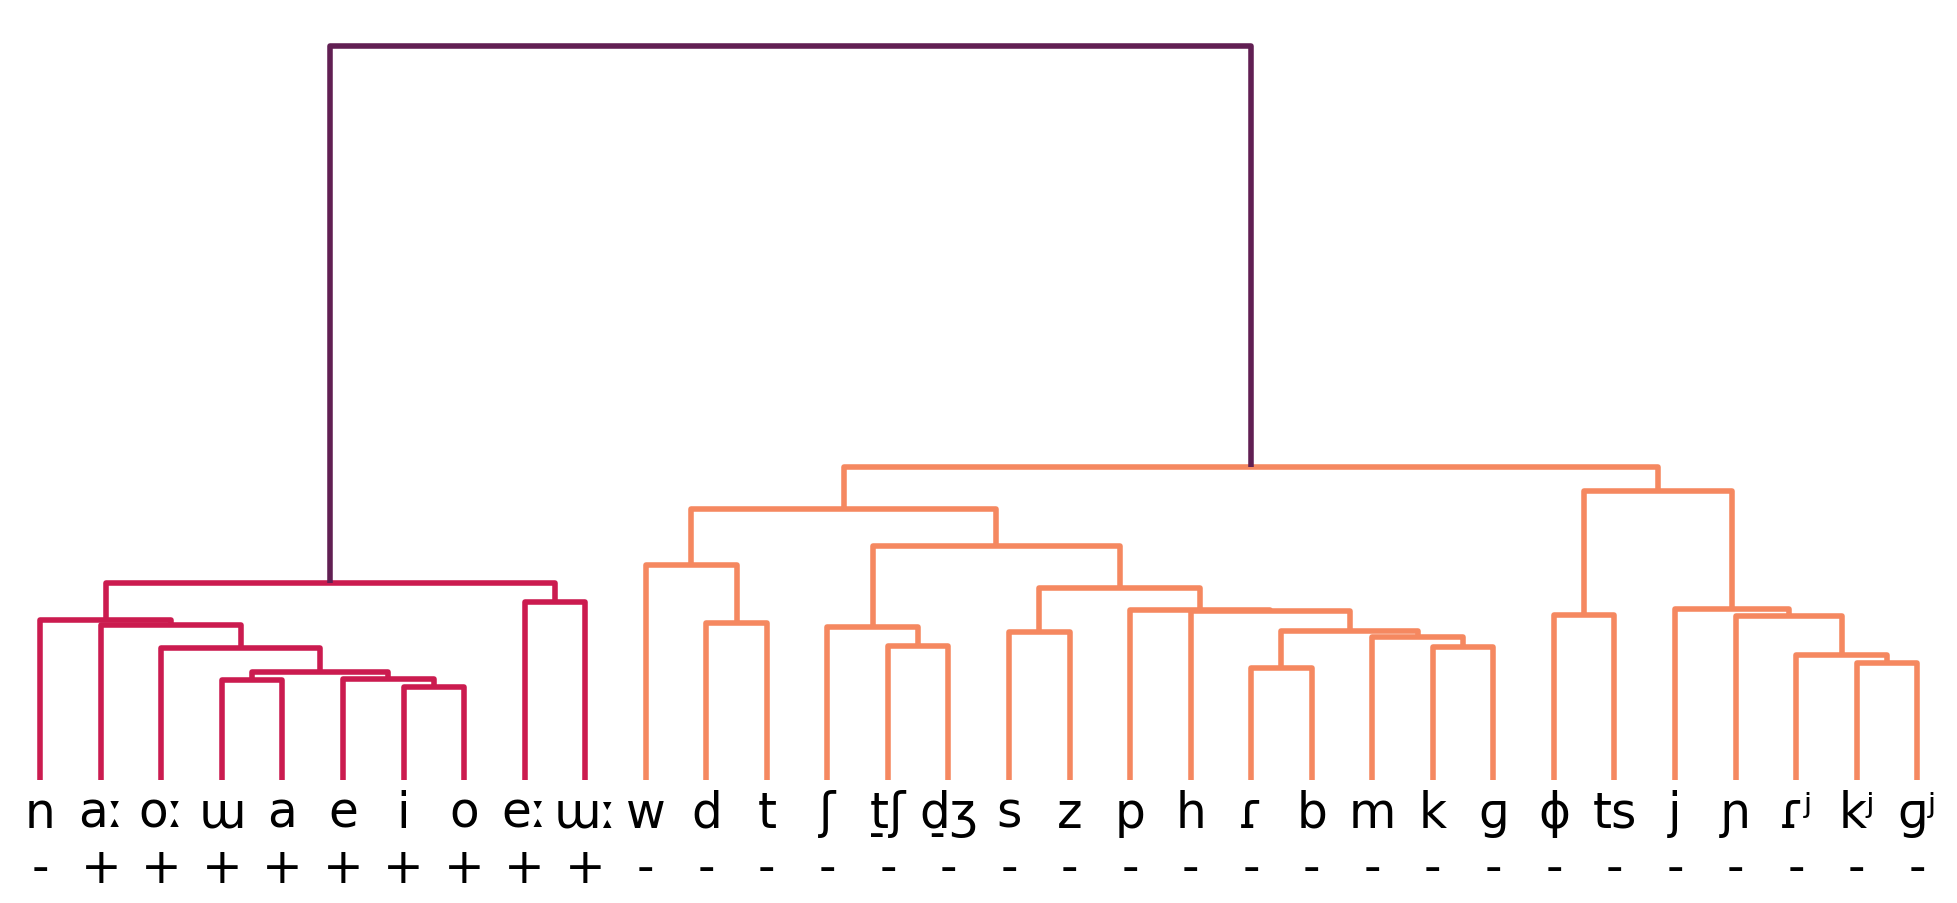
\includegraphics[width=0.99\linewidth]{15Phonology/japanesedendo.png}
        \caption{Japanese}
    \end{subfigure}
    \begin{subfigure}{0.49\textwidth}
        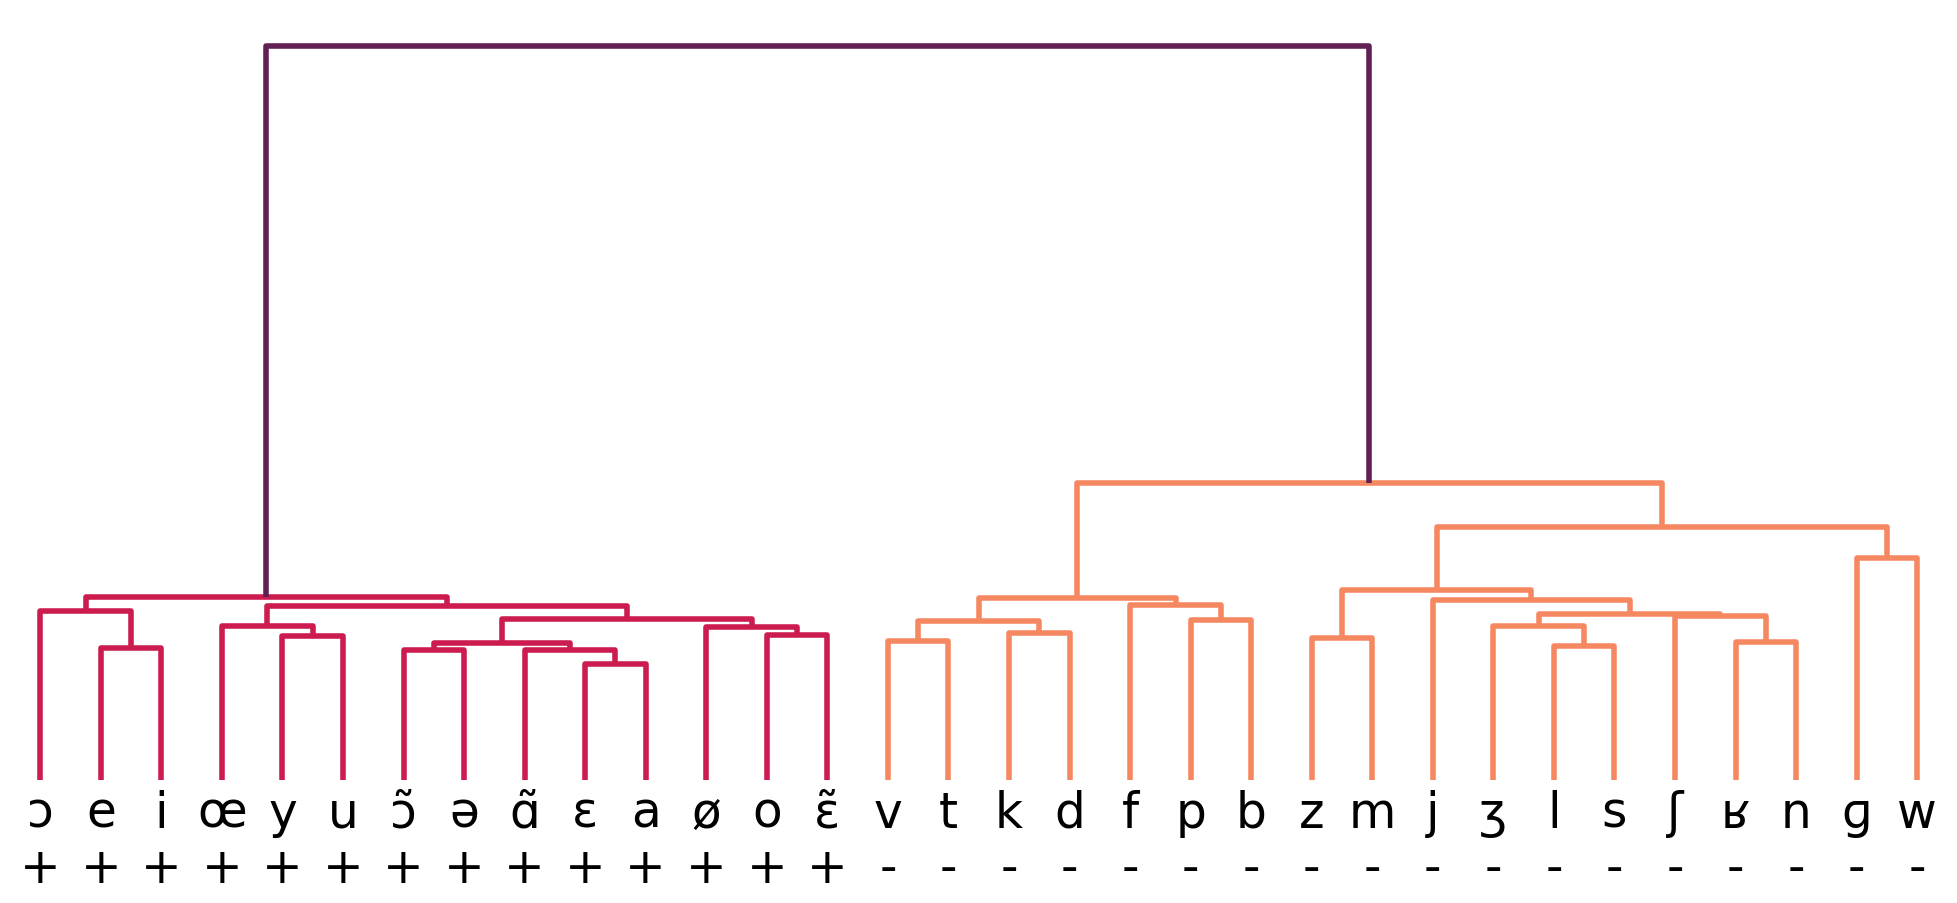
\includegraphics[width=0.99\linewidth]{15Phonology/frenchdendo.png}
        \caption{French}
    \end{subfigure}
    \caption{Similarity of the contextual embeddings for each phoneme learned by the Japanese and French phoneme LMs. Similarities are computed using Euclidean distance considering the average of 50 contextual embeddings for each phoneme and linkages are created using the incremental algorithm. The `syllabic' distinctive feature is marked below each phoneme.} 
    \label{fig:dendrogram}
\end{figure}

The results of each probe are provided in \cref{fig:features}. Statistical significance is assessed using a binomial test, where the null hypothesis assumes a probability of success \( p_0 = 0.5 \) and the number of trials \( n \) is equal to the number of phonemes tested by the probe. A result is considered significant if the computed \( p \)-value is less than 0.05.

The majority of the probes achieve accuracies significantly higher than chance (50\%), indicating that the models learn representations that encode distinctive features. While the scores for each feature are broadly consistent across languages, some notable differences emerge. For example, nearly all feature probes achieve statistically significant results in Mandarin, whereas only two do so in Spanish. This disparity can be partly attributed to the number of unique phonemes in each language. Because each combination of vowel and tone acts as a distinct phoneme, Mandarin has 99 phoneme types, compared to just 24 in Spanish. The smaller phoneme inventory in Spanish greatly reduces $n$ for each probe, making it more challenging to obtain statistically significant results.

In all 11 languages, the highest result is achieved by the probe for the \texttt{syllabic} feature which generally\footnote{In some languages there are also syllabic consonants, which like vowels can act as the nucleus of a syllable.} separates vowels from consonants. As these models only learn to predict phonemes and have no concept of how each phoneme is pronounced, the fact that this separation is learned clearly indicates that vowels and consonants provide a strong distributional signal across languages. The \texttt{consonantal} feature similarly separates vowels from consonants and is learned by a probe in every language. However, not every feature can be learned by these probes. For instance, the \texttt{delayedRelease} feature, which distinguishes stops from affricates, is not learned by any probe. Using a phoneme-based input representation means that the phoneme LMs do not encode the rate of phoneme delivery, so it is unsurprising that a feature that relates to the temporal properties of phonemes is not able to be extracted from the contextual embeddings.

\subsection{Distributional phoneme clusters}

To better understand why the probes capture certain distinctive features, clustering operations can be used to analyse the contextual embeddings of phonemes. For each language, 50 contextual embeddings per phoneme are sampled and labelled them with their associated distinctive features. For each labeling, the \textbf{silhouette score} is computed for each embedding --- a metric ranging from –1 to 1, where higher values indicate that an embedding is more similar to others in its assigned cluster than to those in neighbouring clusters \citep{rousseeuw1987}. Averaging these scores across all embeddings produces a single score for each distinctive feature, indicating the extent to which that feature clusters the phoneme representations, as shown in \cref{fig:silhouette}.

The scores are all relatively close to zero, likely due to the curse of dimensionality --- the embeddings have 256 dimensions, far exceeding the number of distinct phonemes in each language. Despite this, the results are consistent with the probe findings: the syllabic feature yields the highest clustering quality.

Clustering can be further visualised using dendrograms, created by averaging the contextual embeddings for each phoneme and applying an incremental clustering algorithm. \Cref{fig:dendrogram} shows examples for Japanese and French, with the syllabic feature marked for each phoneme. In both cases, vowels are almost entirely separated from consonants, with one notable exception: \ttipa{n} in Japanese. There is also some alignment with traditional phoneme groupings (e.g., \ttipa{b} and \ttipa{p}), though overall the dendrograms diverge from standard phonological classifications. This suggests that the distributional behavior of phonemes in context may not neatly align with their articulatory or categorical properties.

\section{Discussion}\label{sec:15-discussion}

In this chapter, phoneme LMs trained on the 31 languages in \ipachildes are probed for phonological knowledge. Linear probes reveal that these models implicitly encode word boundaries and certain distinctive features and novel unsupervised word segmentation methods indicate that prediction-error and utterance boundary probability can be used as cues for grouping phonemes into word-like units. These experiments also show how \gpp provides new avenues for linguistic analysis by ensuring that phonemes produced for each language are consistent with established inventories in \phoible. Below, the broader implications of these findings are discussed.

%We demonstrate this by training linear probes to extract distinctive features from the contextual embeddings of phonemes learned by our monolingual models. We find that certain features (e.g. \texttt{consonantal}) emerge solely from the distributional properties across all 11 languages, while others (e.g. \texttt{delayedRelease}) do not. 

\paragraph{Statistical learning.} This chapter presents a novel use of prediction-error extracted from LMs for unsupervised word segmentation, extending previous work that explicitly calculated these cues using n-gram models \citep{ccoltekin2014explicit, Coltekin2017, goriely2023word}. This also update previous neural models of word recognition \citep{elman-1990-finding, christiansen1998learning} by using modern transformer-based architectures and cross-lingual evaluation. Viewing these models as statistical learners, there is no single cue or strategy consistently yields the best segmentation performance across different model sizes and languages. This is perhaps unsurprising, as many of the cues are highly interrelated (for example, entropy and surprisal often correlate) and all segmentation strategies are grounded in the same underlying principle: identifying boundaries at points of high prediction uncertainty. It is this general principle, rather than any specific cue or strategy, that proves sufficient for segmenting utterances into word-like units. Nevertheless, most cues and strategies perform reasonably well on their own. Previous segmentation models have explored combining multiple distributional cues through unsupervised majority voting \citep{Coltekin2017, goriely2023word}, an approach that could be fruitfully applied to the cues investigated here in future work.

\paragraph{Cross-lingual comparison.} Comparing models across languages is a challenge. This chapter presents novel methods for exploring the phonological representations of phoneme LMs, but there are several confounding factors that inhibit cross-lingual comparison. Firstly, the distribution of phonemes in word-final slots provides a prior not previously accounted for in studies that probed contextual embeddings for word boundary information. Secondly, word length provides a prior for the unsupervised word segmentation strategies, since randomly placing boundaries yields a higher \fscore when words are shorter, which has not previously been accounted for in cross-lingual word segmentation studies. Nevertheless, both the probes and the unsupervised strategies achieve significant scores for all 31 languages, indicating the importance of the distributional cue for learning to segment speech in any language. Finally, the number of unique phonemes in each language varies, altering the statistical power of significance testing for the distinctive feature probes, but certain features are still significant across all 11 languages tested. These findings also highlight the importance of accounting for frequency information as a prior when training probes or comparing models trained on different datasets.

\paragraph{Cross-lingual modelling.} Whereas the experiments in \cref{chapter:modelling} only used English data, here models are trained across 31 languages. Although this chapter presents the most cross-lingual exploration of word segmentation to date (to the best of my knowledge), the language coverage is still limited: the languages compared are predominantly European and Asian, with no languages indigenous to the Americas, Australia or Africa. Probing the phonological representation of phoneme LMs trained on more globally distributed languages should be explored in future work. For example, the Goldfish suite of language models (monolingual models spanning 350 languages, some trained on as little as 5MB of orthographic text \citep{chang2024goldfish}) could be extended to phonemic modality, but this would require suitable phonemic corpora. Here, \ipachildes is used, but if the child-directed constraint is relaxed, other corpora surveyed in \cref{chapter:resources} could be leveraged, such as VoxLingua107 \citep{9383459} or CMU Wilderness \citep{8683536} --- though these would need to be converted to phonemes using a tool like \gpp. Finally, future work could also explore multi-lingual modelling, where IPA has proven to be effective for force-alignment \citep{zhu-etal-2024-taste} and zero-shot cross-lingual NER \citep{sohn2024zero}.

\paragraph{Simulating acquisition.} The results focus on the performance of phoneme LMs at the end of training, whereas past work has compared the learning dynamics of phoneme-based models to developmental patterns observed in human acquisition \citep{kirov-2018-recurrent}. Although the word segmentation results indicate the utility of the distributional cue for identifying word-like units, this thesis does not claim that the phoneme LMs simulate language acquisition. In particular, given recent advances in models that operate directly on raw audio, the use of phoneme-level representations may be insufficient for capturing the full complexity of language learning, as discussed further in \cref{chapter:discussion}. While many computational models of word segmentation treat segmentation as a necessary precursor for language understanding, this assumption has been questioned. For example, \citet{baayen2016} show that a tri-phone model, operating on unsegmented utterances can make predictions consistent with infants' sensitivity to linguistic structure. 

%Rather, we use this framework to investigate the distributional patterns of phonemes across languages and whether language models trained to predict upcoming phonemes implicitly track meaningful sub-sequences that align with words. While many computational models of word segmentation treat segmentation as a necessary precursor for language understanding, this assumption has been questioned. For example, \citet{baayen2016} show that a tri-phone model, operating on unsegmented utterances can make predictions consistent with infants' sensitivity to linguistic structure. Likewise, recent phoneme-level language models perform well on both linguistic benchmarks and downstream tasks without explicit segmentation \citep{goriely2024babble} --- although our results suggest that some degree of implicit segmentation may be occurring to enhance these models' predictive performance. 

\paragraph{Word boundaries as gold labels.} For the word boundary experiments, word boundaries from orthographic text were used as the gold labels for evaluation, but these boundaries may not correspond with lexical units in speech. In early stages of acquisition, children may treat both predictable multi-word phrases as single lexical units \citep{macwhinney1978} and unsupervised word segmentation strategies may be segmenting morphemes, rather than words \citep{fleck2008lexicalized}. From an information-theoretic angle, word boundaries may only exist to optimise the trade-off between syntax and morphology across languages \citep{koplenig2017statistical, mosteiro2025word} and in general, what exactly defines a `word' is still up for debate \citep{dixon2002word, haspelmath2023defining}. 

\paragraph{Unsupervised segmentation for tokenisation.} Instead of evaluating against word boundaries, the unsupervised segmentation cues can be treated as \emph{graded} measures of co-occurrence statistics, as noted by \citet{elman-1990-finding}. This idea can be leveraged to improve the tokenisation step in modern LM training. Instead of forming subwords by merging frequently occurring byte pairs, token sequences that are highly predictable can be combined, similar to the constraints used in modern patching methods discussed in \cref{sec:12-alternative}. This idea is used to motivate a new subword tokenisation method introduced in \cref{chapter:infotokenisation}. 

%\citet{pagnoni2024byte} apply this concept to a ``token-free'' model, where bytes are joined into `patches' according to the entropy of the probability distribution for each byte (probabilities are computed using a byte-level LLM). They use two constraints for merging bytes which exactly correspond to our threshold and relative segmentation strategies, but only use entropy as a cue. In our experiments, entropy was less effective than utterance boundary probability (UBP) for unsupervised word segmentation and in an initial investigation (see \cref{app:tokenizers}) we found that creating a subword tokenizer using both cues improves the linguistic abilities of models trained on phonemes compared to regular BPE and that the UBP cue is more effective than entropy. This creates a parallel between word segmentation research and practical applications for tokenization in NLP and we encourage further work in this area.

%which we found to be inferior to utterance boundary prediction and model loss for unsupervised word segmentation. In an initial investigation (see \cref{app:15-tokenizers}), we found that tokenizers based on these cues improve the linguistic abilities of models trained on phonemes over regular BPE, creating a link between word segmentation research and tokenization in NLP. We encourage future work to further explore the use of these cues to improve tokenization.

\section{Summary}

This chapter has primarily contributed to Research Question \ref{question:rq2} by demonstrating that phoneme LMs trained on developmentally plausible corpora are a valuable tool for cross-lingual phonological experimentation. Word boundary and distinctive feature probes are utilised to investigate the phonological representations learned by these models and novel unsupervised word segmentation methods are introduced, leveraging prediction-error and utterance boundary probability to identify words. These also contribute to \ref{question:rq1}, as language-agnostic methods for evaluating phoneme LMs. 

These methods indicated that phoneme LMs trained on 31 languages can all detect word boundaries and that models certain features (e.g. \texttt{consonantal}) emerge solely from the distributional properties across 11 languages, while others (e.g. \texttt{delayedRelease}) do not. This study also revealed how cross-linguistic comparisons are influenced by confounding factors such as word length, word-final phoneme distribution and inventory size. These factors, while positing challenges, also offer new avenues for understanding the role of distributional cues in language processing cross-lingually.

The phonological experimentation conducted in this chapter can also provide insights into how language models learn, contributing to Research Question \ref{question:rq3}. Here, small LMs trained to predict phonemes without word boundaries implicitly track word boundary information, likely to improve future predictions. This could explain why although scoring lower than LMs trained with word boundaries, the models trained in the input representation experiment presented in \cref{sec:14-phonemepretraining} still perform competitively on BLiMP and GLUE --- the models leverage distributional information to implicitly group word-like units to succeed at grammatical and language understanding benchmarks. The unsupervised word segmentation methods presented in this chapter also have similarities to subword tokenisation methods --- a connection further explored in \cref{chapter:infotokenisation}, highlighting how this research can inform and improve practical applications in natural language processing.

% From ipa childes
% We demonstrate the utility of these resources for phonological analysis using phoneme LMs by extending prior work to the cross-lingual setting. Our results establish the corpus size requirements for phoneme LMs trained on developmentally plausible corpora and we show that models trained on 11 languages effectively implicitly encode distinctive features. These findings support the role of phoneme LMs in studying emergent phonology. 


% \section{Limitations}\label{app:15-limitations}

% We acknowledge the following limitations of our work.

% \paragraph{Limitations of phonemic data:} Using phonemic data for the word segmentation task is the typical framework for exploring relevant acquisition theories. However, the phonemic transcriptions in \ipachildes do have limitations. Having been generated using grapheme-to-phoneme (G2P) conversion, they may have been subject to conversion error, and the original transcriptions may also contain errors. The G2P process also removes natural variation in speech, such as accents and allophonic variation. The symbolic nature of phonemes may also be an unrealistic starting point for acquisition; it is unclear if infants have access to phonetic categories at this stage of acquisition \citep{feldman_infants_2021, mcmurray_myth_2022}. Researchers who advocate for using language models as cognitive models argue that the training data should be as developmentally plausible as possible \citep{dupoux-2018-cognitive, warstadt-2022-artificial}, and that phonemes may be as implausible as text for simulating early acquisition \citep{lavechin}.

% From this perspective, a more appropriate framework is to learn segmentation directly from raw audio, as pursued in the Zero Resource Speech Challenge \citep{nguyen2020zero, dunbar2021zero}. Audio-based models naturally incorporate prosodic cues, which play a key role in language acquisition \citep{Cutler1987, Jusczyk1993stress, jusczyk-1999-stress-voice}. Unsupervised models have demonstrated the ability to perform statistical learning directly from raw speech \citep{lavechin2022can, seyssel-2023-realistic}, and have found that the resulting units tend to be shorter than phonemes, consistent with early perceptual categories \citep{schatz2021early}. While such models show promising signs of early phonetic learning and perform well on word-level tasks, they currently require significantly more data to match the performance of text-based models \citep{lavechin}. Moreover, training on curated audiobook datasets gives these models a considerable advantage over learning from noisier, long-form audio that better resembles real-world input—but ongoing work is making such realistic simulations increasingly viable \citep{lavechin2024modeling}.

% \paragraph{Distribution of languages:} When training models cross-lingually, we were limited by the scale of each language partition of the \ipachildes dataset. The dataset has a very skewed distribution: the EnglishNA section contains 18M words but the Farsi section only contains 43k words. We addressed this skew by training four suites of models in order to provide a cross-lingual comparison while also exploring how segmentation performance increased in scale for the languages with more data available.

% \paragraph{Language coverage:}
% To the best of our knowledge, our work is the most cross-lingual exploration word segmentation to date, but is still limited in language coverage: the languages we compare are predominantly European and Asian, with no languages indigenous to the Americas, Australia or Africa. Word segmentation of languages that are more globally distributed should be explored in future work.

% \section{Using word segmentation cues for subword tokenization}\label{app:15-tokenizers}

% We briefly explore the use of our unsupervised word boundary cues to create a subword tokenizer. Typically, the vocabularies for these tokenisers are generated using methods like Byte-Pair Encoding \citep{sennrich-etal-2016-bpe}, where the vocabulary initially consists of each individual byte, and pairs of bytes that frequently co-occur in a training dataset are `merged' into a new token, with this process repeated until a fixed vocabulary size is reached. We use the same principle, but base merges on the word boundary cues from a language model trained on the dataset.

% Our method is as follows:

% \begin{enumerate}
%     \item We take a trained phoneme-level LM and compute either the UBP cue or the entropy cue at every position in the a given dataset. 
%     \item We initialise our vocabulary $V$ to match the vocabulary of the phoneme LM (so it contains every phoneme plus the utterance boundary token).
%     \item For every pair of tokens $x_i, x_j \in V$ that co-occur in the dataset, we compute the score for that pair by finding the average value of the word boundary cue at the position of the second token in the pair (e.g. for the pair \ttipa{D,E}, we find the value of the cue at every position where \ttipa{E} appears after \ttipa{D} and return the average). 
%     \item We find the pair with the lowest score, create a new token $V_i+V_j$, add it to the vocabulary and apply the merge to every token in the dataset. The cue's value at the newly merged token is set to be the sum of the cue's value of the two tokens before the merging occurs. For the entropy cue this follows from the chain rule and for the UBP cue this results in the probability that \emph{either} original token was an utterance boundary.
%     \item We repeat (2)-(3), adding new tokens and applying merges until a fixed vocabulary size is reached.
% \end{enumerate}

% Conceptually, creating merges using minimum average entropy will join highly predictable tokens together and result in tokens with comparable information and a uniformly dense signal that the model can learn from. Creating merges using the minimum average probability of an utterance boundary is similar, but instead tokens are joined according to the model's certainty that they do not cross an utterance boundary. 

% In order to test this method, we use the phoneme-level LM trained by \citet{goriely2024babble} on a phonemized\zeb{fix?} version of the 100-million word BabyLM dataset \citep{choshen-et-al-2024-callforpapers-babylm2} and train subword tokenizers using a phonemized version of the 10-million word BabyLM dataset. We create two tokenisers with a vocabulary size of 16k using the UBP cue and the entropy cue. We compare these to the BPE tokeniser trained by \citet{goriely2024babble} on the same dataset, which also has a vocabulary size of 16k. Note that all three tokenisers are trained on a dataset without word boundaries, so it is possible for tokens to span word boundaries.

% \citet{goriely2024babble} trained a large model using their BPE tokeniser on the 100-million word BabyLM dataset and evaluated their results on two linguistic benchmarks, BLIMP \citep{warstadt-2020-blimp} and BabySLM \citep{lavechin}. We train and evaluate a model using the same procedure but replace their tokeniser for ours. 

% \begin{table}[t]
%     \centering
%     \begin{tabular}{lccc}
%         \toprule
%         Tokeniser & \rotatebox[origin=l]{90}{BLIMP} & \rotatebox[origin=l]{90}{BabySLM Syntactic} & \rotatebox[origin=l]{90}{BabySLM Lexical} \\
%         \midrule
%         BPE & 71.7 & 74.7 & 71.2 \\
%         Entropy & 72.7 & 77.6 & 81.3 \\
%         UBP & 72.6 & 85.6 & 84.4 \\
%         \bottomrule
%     \end{tabular}
%     \caption{BLIMP and BabySLM scores achieved by a GPT-2 model trained on the BabyLM dataset. We compare BPE to our subword method, where merges are assigned using either entropy or UBP as a cue. BPE results are taken from \citet{goriely2024babble}.}
%     \label{tab:15-tokeniserresults}
% \end{table}

% The results of this experiment are provided in \cref{tab:15-tokeniserresults}. We find that our two tokenisers improve all three scores compared to the BPE but instead tokeniser with the UBP cue leading to a particularly large improvement for the BabySLM syntactic score.

% Our method is similar to \citet{pagnoni2024byte}, who calculate the entropy cue over bytes using a small byte-level LLM, and use either a \textit{global constraint} (corresponding to our threshold segmentation strategy) or a \textit{monotonic constraint} (corresponding to our relative segmentation strategy) in order to group bytes into latent `patches'. These patches are then fed into the main model, a large transformer, and the encoded patches are `unpatched' and fed back into the byte-level LLM to predict the next byte. Future work should investigate whether their method is improved by using the cues explored in this study. When training with word boundaries, the prediction of the space character (or other word boundary characters) could also be used to group bytes.


% Copied from ipa childes paper


% Our resources could also support the training of self-supervised speech models \citep[e.g.][]{hsu2021hubert}. These models are trained directly on audio and lag behind phoneme or text-based models, often requiring several orders of magnitude more data to learn semantic representations \citep{cuervo2024scaling}, but recent work has found that fine-tuning on phoneme classification can reduce this gap \citep{feng-2023-language-universal-phonetic, poli2024improving}. 
